\documentclass[10pt, a4paper]{article} %or article has only section and below, book and report also have chapter: http://texblog.org/2007/07/09/documentclassbook-report-article-or-letter/
\usepackage{float}
\usepackage[babel,german=quotes]{csquotes}%nice quotations
\usepackage[utf8]{inputenc} % use utf8 encoding of symbols such as umlaute for maximal compatibility across platforms
\usepackage{caption} % provides commands for handling caption sizes etc.
\usepackage[a4paper, left=30mm, right=30mm, top=25mm, bottom=20mm]{geometry} % to easily change margin widths: https://www.sharelatex.com/learn/Page_size_and_margins
\usepackage[bottom]{footmisc} % I love footnotes! And they should be down at the bottom of the page!
\usepackage{graphicx,subfig} % when using figures and alike
\usepackage[hidelinks]{hyperref} % for hyperreferences (links within the document: references, figures, tables, citations)
\usepackage{euler} % a math font, only for equations and alike; call BEFORE changing the main font; alternatives: mathptmx, fourier,
%\usepackage{gentium} % for a different font; you can also try: cantarell, charter, libertine, gentium, bera, ... http://tex.stackexchange.com/questions/59403/what-font-packages-are-installed-in-tex-live
%------------------------------------------------------------------------------------------------------
%------- text size settings --------------
\setlength{\textwidth}{16cm}%
\setlength{\textheight}{25cm} %23
%(these values were used to fill the page more fully and thus reduce the number of pages!)
\setlength{\topmargin}{-1.5cm} %0
\setlength{\footskip}{1cm} %
%\setlength{\hoffset}{0cm} %
%\setlength{\oddsidemargin}{1cm}%
%\setlength{\evensidemargin}{-.5cm}%
\setlength{\parskip}{0cm} % Abstand zwischen Absätzen
% ----------------------------------------------------------------
\renewcommand{\textfraction}{0.2} % allows more space to graphics in float
\renewcommand{\topfraction}{0.85}
%\renewcommand{\bottomfraction}{0.65}
\renewcommand{\floatpagefraction}{0.70}
\frenchspacing %http://texwelt.de/wissen/fragen/1154/was-ist-french-spacing-was-macht-frenchspacing
%------------------------------------------------------------------------------------------------------
%------------------------------------------------------------------------------------------------------

\usepackage{Sweave}
\begin{document}
\Sconcordance{concordance:FINAL_VERSION.tex:FINAL_VERSION.Rnw:%
1 31 1 1 0 11 1 1 6 77 1 1 2 5 0 1 2 5 1 1 2 1 0 1 1 %
4 0 1 2 76 1 1 14 13 0 11 1 1 2 3 0 1 2 6 1 1 6 1 25 %
27 0 1 2 3 1 1 5 1 23 25 0 1 2 3 1 1 2 1 0 6 1 3 0 1 %
2 7 1 1 3 2 0 1 1 1 2 1 0 1 1 1 3 2 0 2 1 1 2 1 0 5 1 %
1 2 5 0 1 2 5 1 1 2 17 0 1 2 5 1 1 2 21 0 2 2 1 0 1 1 %
2 0 1 1 3 0 1 2 6 1 1 2 1 0 1 2 1 0 3 1 1 2 5 0 1 2 7 %
1 1 4 15 1 1 4 3 1 1 4 4 1 1 4 19 1 1 4 9 1 1 2 4 0 1 %
3 4 0 1 2 4 1 1 4 3 1 1 4 8 1 1 2 4 0 1 2 3 1 1 4 3 1 %
1 4 12 1 1 12 14 0 1 2 2 1 1 2 4 0 1 2 32 1 1 2 1 0 1 %
1 3 0 2 2 4 0 1 2 4 1 1 4 3 1 1 4 11 1 1 2 1 0 4 1 1 %
4 4 1 4 0 1 3 1 2 1 0 4 1 3 0 1 2 3 1 1 2 18 0 2 2 10 %
0 1 2 5 1 1 4 3 1 1 4 9 1 1 2 1 0 1 3 2 0 1 1 3 0 2 2 %
4 0 1 2 3 1 1 4 3 1 1 4 6 1 1 2 1 0 1 3 5 0 1 2 11 1 %
1 2 3 0 1 1 3 0 1 2 2 1 1 5 4 0 1 4 7 0 1 2 8 1 1 2 1 %
0 1 4 3 0 1 1 3 0 1 2 5 1 1 6 5 0 1 1 1 6 4 0 1 1 3 0 %
2 2 1 0 1 1 3 0 2 2 6 0 1 1 9 0 1 3 14 1 1 2 1 0 1 3 %
2 0 1 3 6 0 1 2 9 1 1 4 3 1 1 4 3 1 1 4 6 1 1 2 10 0 %
1 2 1 1 1 4 11 1 1 2 1 0 1 2 1 0 1 1 6 0 1 2 5 1 1 7 %
11 0 1 2 13 1 1 2 13 0 1 2 2 1 1 2 1 0 4 1 4 0 1 2 6 %
1 1 2 4 0 1 2 4 1 1 4 3 1 1 4 3 1 1 4 7 1 1 4 8 1 1 2 %
10 0 1 2 21 1 1 2 1 0 4 1 1 4 3 0 1 2 1 0 2 1 3 0 1 2 %
1 4 3 0 10 1 1 2 5 0 1 2 5 1 1 2 1 0 1 1 3 0 2 2 1 0 %
1 1 3 0 1 2 1 1 1 2 1 0 2 1 4 0 1 2 3 1 1 2 4 0 1 2 8 %
1 1 4 3 1 1 4 9 1 1 2 11 0 1 1 11 0 1 3 5 1 1 2 1 0 2 %
1 4 0 1 2 7 1 1 2 1 0 1 1 12 0 1 2 7 1 1 2 4 0 2 2 1 %
0 1 1 4 0 1 2 1 6 5 0 1 1 3 0 1 2 2 1 1 2 8 0 1 5 10 %
1 1 2 5 0 1 2 1 1 1 2 1 0 1 1 3 0 1 2 6 1 1 2 1 0 2 1 %
5 0 1 3 5 1 1 2 11 0 1 1 10 0 1 2 5 1 1 2 1 0 1 1 22 %
0 1 1 8 0 1 2 2 1 1 2 1 0 2 1 4 0 1 2 3 1 1 2 1 0 1 1 %
3 0 2 2 4 0 2 2 32 0 1 1 8 0 1 2 2 1 1 2 6 0 1 2 4 1 %
1 2 5 0 1 2 4 1 1 2 10 0 1 2 28 1 1 2 1 0 1 2 1 0 1 1 %
5 0 1 3 4 1 1 2 1 0 1 1 5 0 1 3 5 1 1 2 1 0 2 1 12 0 %
1 3 5 1 1 2 1 0 3 1 4 0 1 2 9 1 1 2 1 0 2 1 5 0 1 3 5 %
1 1 2 1 0 1 1 10 0 1 2 5 1 1 2 1 0 2 1 4 0 1 2 4 1 1 %
2 1 0 1 1 6 0 1 2 5 1 1 2 1 0 1 1 11 0 1 2 2 1 1 2 1 %
0 1 1 1 2 1 0 1 2 1 0 1 2 1 0 1 1 1 2 1 0 1 1 1 4 3 0 %
1 1 5 0 1 3 5 1 1 2 1 0 1 1 5 0 1 3 4 1 1 2 1 0 1 2 5 %
0 1 2 10 1 1 2 1 0 2 2 1 0 1 1 1 3 2 0 1 2 5 0 1 2 5 %
1 1 2 1 0 2 1 1 2 5 0 1 2 3 1 1 2 6 0 1 1 5 0 1 1 5 0 %
1 1 6 0 1 2 31 1}

\setkeys{Gin}{width=0.6\textwidth}
\title{Time Series Analysis - A Tutorial \\
for Temporally Correlated Time Series}
\author{Rosskopf,E.; Cordes, M.; Lumiko, J.}
% for more control, multiple affiliations, line breaks and alike, use the authblk package!!
\date{\today} % !!use package isodate for more control of date formatting!!
\maketitle
\tableofcontents
\pagebreak


\section{Introduction}%------------------------------------------------------------------------------------
\noindent This tutorial assumes that the reader has some basic knowledge of time series analysis, and the principal focus of the tutorial is not to explain time series analysis, but rather to explain how to carry out these analyses using R.\\
\\This chapter covers some fundamental theory and is meant to give you a better understanding about the following chapters that give attention to the analysis of time series. 

\subsection{Definition}
\noindent A time series is a record of values of a certain variable of interest taken at different points in time. Data are observed at equally spaced time intervals (Discrete time series) and the method of measurement is supposed to be consistent over time.\\

\subsection{Applications}

\noindent Depending on the field of work, time series analysis can be useful for several applications.\\

\noindent \textbf{Geosciences and meteorology}\\
\begin{itemize} 
\item Weather forecasting, trends in weather patterns\\
\end{itemize}
\\
\textbf{Business and finance (econometrics)}\\
\begin{itemize} 
\item Stock market analysis, business forecasting\\
\end{itemize} 
\noindent \textbf{Multivariate statistical data analysis}\\
\begin{itemize} 
\item RS image analysis\\
\end{itemize} 
\textbf{Medicine}\\
\begin{itemize}
\item Epidemic analysis
\end{itemize}


\subsection{Goals depending on the study question}%---------------------------

\textbf{Climatologist interested in global warming}\\
\begin{itemize}
\item Interested in the long term trend of CO2 or temperature, thus ignoring the daily/monthly/seasonal cycles\\
\end{itemize}
\textbf{Economist interested in demand for electricity}\\
\begin{itemize}
\item Interested in the long term trends(due to population growth? Global warming?) but also the daily/monthly/seasonal peaks\\
\end{itemize}
\textbf{Epidemiologist interested in preparing for the flu season}\\
\begin{itemize}
\item  Not really interested in long term trends, the focus is set more on monthly/seasonal cycles and errors (abnormal spikes in the flu rates)
\end{itemize}

\pagebreak

\subsection{Decomposition}%---------------------------
Decomposing a time series means separating it into its constituent components, which are usually a trend component and an irregular component, and if it is a seasonal time series, a seasonal component:\\

\noindent 1.) \textbf{Trend}\\
\\
2.) \textbf{Cycles} (including seasonal)\\
\\
3.) \textbf{Irregular components}\\
\\
These components can be described as follows:\\
\\
\\
\noindent {\Large X}t{\Large = T}t{\Large +S}t{\Large +C}t{\Large +R}t\\
\\
\\
\noindent where:\\
\\
\textbf{Xt} = Value of the series at time t\\
\textbf{Tt} = trend component of the series\\
\textbf{St} = Cyclical or seasonal component with a period S\\
\textbf{Rt} = Random effect for which we have no explanation\\
\\
\textbf{Note: This idea is very old and is now out of favor but it is still widely used}
\\
\\
\\
\textbf{Example: Decomposition of monthly deaths from lung diseases in the UK}
\\
\begin{figure}[h]
\centering
\begin{Schunk}
\begin{Sinput}
> plot(ldeaths)
\end{Sinput}
\end{Schunk}
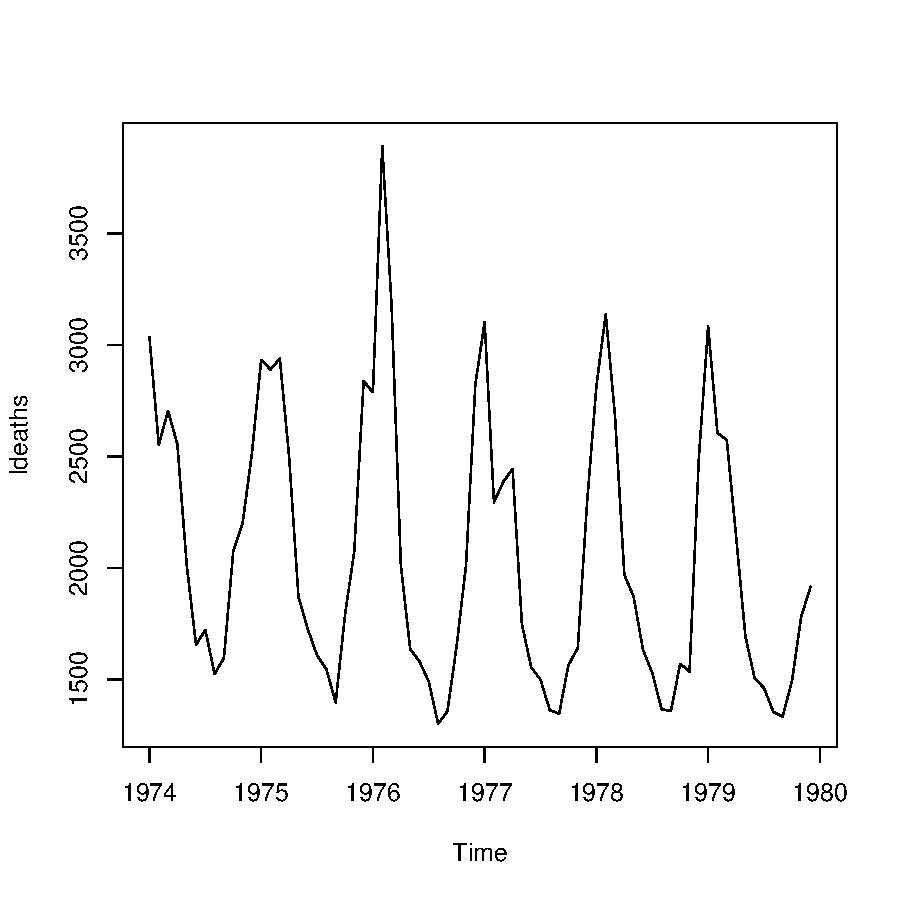
\includegraphics{FINAL_VERSION-Deathplot}
\caption{Plot of monthly deaths from lung diseases in the UK}
\end{figure}
\\

\begin{figure}[H]
\centering
\begin{Schunk}
\begin{Sinput}
> ldeathcomponents = decompose(ldeaths)
> plot(ldeathcomponents)
\end{Sinput}
\end{Schunk}
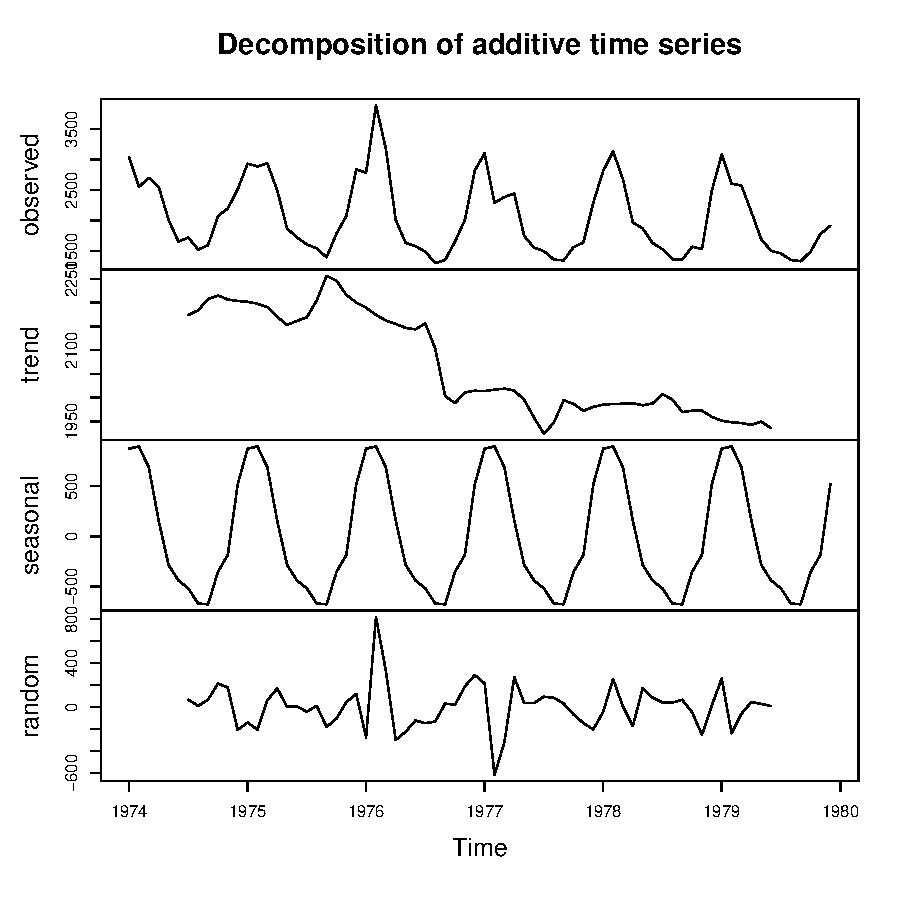
\includegraphics{FINAL_VERSION-Decomposition}
\caption{Decomposition of monthly deaths from lung diseases in the UK}
\end{figure}

\subsubsection{Decomposing Seasonal Data}%---------------------------------------------------------------

A seasonal time series consists of a \textbf{trend component}, a \textbf{seasonal component} and an \textbf{irregular component}. Decomposing the time series means separating the time series into these three components: that is, estimating these three components.\\

\noindent To estimate the trend component and seasonal component of a seasonal time series that can be described using an additive model, we can use the \textbf{“decompose()”} function in R. This function estimates the trend, seasonal, and irregular components of a time series that can be described using an additive model.\\
\\
\noindent The function “decompose()” returns a list object as its result, where the estimates of the seasonal component, trend component and irregular component are stored in named elements of that list objects, called “seasonal”, “trend”, and “random” respectively.\\
\\


\subsection {Stationarity and differencing}%---------------------------------------------------------------
\noindent A stationary time series is one whose statistical properties such as \textbf{mean, variance, autocorrelation, etc.} are all \textbf{constant over time}. Most statistical forecasting methods are based on the assumption that the time series can be rendered approximately stationary (i.e., "stationarized") through the use of mathematical transformations.\\

 A \textbf{stationarized series} is relatively \textbf{easy to predict}: you simply predict that its \textbf{statistical properties will be the same in the future as they have been in the past!} The predictions for the stationarized series can then be "untransformed," by reversing whatever mathematical transformations were previously used, to obtain predictions for the original series. (The details are taken care of by R.) \\
 \\
Thus, finding the sequence of transformations needed to stationarize a time series often \textbf{provides important clues in the search for an appropriate forecasting model}.  Stationarizing a time series through \textbf{differencing} (where needed) is an important part of the process of fitting an ARIMA mode.\\
\\
Another reason for trying to stationarize a time series is to be able to obtain \textbf{meaningful sample statistics} such as means, variances, and correlations with other variables. Such statistics are useful as \textbf{descriptors of future behavior} only if the series is stationary.\\
\\
 For example, if the \textbf{series is consistently increasing over time}, the sample mean and variance will grow with the size of the sample, and they will \textbf{always underestimate the mean and variance in future periods}. And if the mean and variance of a series are not well-defined, then neither are its correlations with other variables. \textbf{For this reason you should be cautious about trying to extrapolate regression models fitted to nonstationary data.}
\\
Most business and economic time series are far from stationary when expressed in their original units of measurement, and even after deflation or seasonal adjustment they will typically still exhibit trends, cycles, random-walking, and other non-stationary behavior.\\
\\
If the series has a stable long-run trend and tends to revert to the trend line following a disturbance, it may be possible to stationarize it by de-trending (e.g., by fitting a trend line and subtracting it out prior to fitting a model, or else by including the time index as an independent variable in a regression or ARIMA model), perhaps in conjunction with logging or deflating.\\
\\
Such a series is said to be trend-stationary. However, sometimes even de-trending is not sufficient to make the series stationary, in which case it may be necessary to transform it into a series of period-to-period and/or season-to-season differences.  If the mean, variance, and autocorrelations of the original series are not constant in time, even after detrending, perhaps the statistics of the changes in the series between periods or between seasons will be constant.\\
\\   
Such a series is said to be difference-stationary.  (Sometimes it can be hard to tell the difference between a series that is trend-stationary and one that is difference-stationary, and a so-called unit root test may be used to get a more definitive answer.)

\subsubsection{How to make a series X stationary}%---------------------------------------------------------------

\textbf{1.) Check if there is variance that changes with time}\\
\begin{itemize}
\item Make variance constant with log or square root transformation\\
\item Call the transformed data X*\\
\end{itemize}
\noindent \textbf{2.) Remove the trend in mean with regular differencing or fitting a trend line}\\
\begin{itemize}
\item Call the new series X**\\
\item The correlogram of X** should only have a few significant spikes at small lags\\
\end{itemize}
\noindent \textbf{3.) If there is seasonal cycle left in the data, we must seasonally difference the series too}\\
\begin{itemize}
\item Call the new series X**\\
\end{itemize}

\pagebreak
\subsection{Important terminology}%---------------------------------------------------------------

\textbf{Dependence}\\
\\
Correlation of observations of one variable at one point in time with observations of the same variable at prior points in time \textbf{(Serial correlation / autocorrelation)}\\
\\
\textbf{Stationarity}\\
\\
The \textbf{mean and variance} of the series \textbf{remains constant} over the time series (e.g., no systematic change in the mean, no trend)\\
\\
\textbf{Differencing}\\
\\ 
Data pre-processing step which de-trends the data to achieve stationarity\\

\noindent \textbf{Specification}\\

\noindet Using \textbf{diagnostic tests}, specifying the type of time series model to apply to the series\\
\begin{itemize}
\item{Auto-regressive(AR), Moving average (MA), ARMA (combined) or ARIMA (combined integrated)}\\
\item{Non linear models also possible}
\end{itemize}
\pagebreak

\section{Getting started}%------------------------------------------------------------------------------------
\subsection{Packages}
Before we get started, please make sure to set a working directory and download the necessary packages listed below.\\
\noindent Useful packages for time series analysis:
\begin{Schunk}
\begin{Sinput}
> #install.packages(tseries)
> #install.packages(nlme)
> #install.packages(car)
> #install.packages(knitr)
> #install.packages(xtable)
> #install.packages(SweaveListingUtils)
> #install.packages(stats)
> #install.packages(forecast)
> #install.packages(AICcmodavg)
> #install.packages(TTR)
> #install.packages(mgcv)
> 
> library(tseries)
> library(nlme)
> library(car)
> library(knitr)
> library(xtable)
> library(SweaveListingUtils)
> library(stats)
> library(forecast)
> library(AICcmodavg)
> library(TTR)
> library(mgcv)
> library(dlm)
> setwd("//csrv05/public$/Elenamarlene/BestpracticeR/timeseries/FINAL_VERSION/")
\end{Sinput}
\end{Schunk}


\subsection{Applied functions}
\noindent It saves time and makes it easier to follow the tutorial, if the largest functions are placed first. If they apply lateron, they can simply be written in one line without losing focus. \\
The first function assembles necessary tests, we need iteratively to run after we changes a model structure.  The performed function is a diagnostic check wie need to perform in order to revise if our model is adequate enough to stop the model adaptation. We need to be careful if we want to check for residuals or the fitted values so it will be specified in the function \emph{diagnostics}.
\\


\begin{Schunk}
\begin{Sinput}
> diagnostics <- function (x)
 {
 normality = signif(shapiro.test(x$residuals)$p.value); #check for normal distributed values #
 stat.res = adf.test(x$residuals); #check both residuals
 #of the model for stationarity
 stat.res =signif(adf.test(x$residuals)$p.value);
 stat.res.alt = adf.test(x$residuals)$alternative;
 x$residualsvector = as.vector(x$residuals);
 autocorr= dwt(x$residualsvector) ; #check for autocorrelation
 indep= signif(Box.test(x$residuals, type="Ljung-Box")$p.value) #check for independence
 #lag for season is df: m-1 ( 12-1)
 #write if seasonal = TRUE lag=12-1, else write nothing
 #there is high evidence that there are non-zero autocorr.
 c1= cbind(normality, stat.res, stat.res.alt, autocorr, indep);
 c2 = c("normal distribution of residuals",
        "stationarity of residuals",
        "alternative stationarity type",
        "autocorrelation of residuals",
           "independence of residuals");
 
 matrix = as.matrix(c1,c2, desparse.level=1);
 
 return ( matrix )
 }
\end{Sinput}
\end{Schunk}
\noindent The next function compiles \emph{plotForecastErrors}
the visualization of the distribution of the errors of a forecast function and overlays it with a normally distributed data to depict mistakes in therespective forecast functions. 



\begin{Schunk}
\begin{Sinput}
> plotForecastErrors <- function(forecasterrors)
 {
 # make a histogram of the forecast errors:
 mybinsize <- IQR(forecasterrors)/4
 mysd <- sd(forecasterrors)
 mymin <- min(forecasterrors) - mysd*5
 mymax <- max(forecasterrors) + mysd*3
 # generate normally distributed data with mean 0 and standard deviation mysd
 mynorm <- rnorm(10000, mean=0, sd=mysd)
 mymin2 <- min(mynorm)
 mymax2 <- max(mynorm)
 if (mymin2 < mymin) { mymin <- mymin2 }
 if (mymax2 > mymax) { mymax <- mymax2 }
 # make a red histogram of the forecast errors, with the normally distributed data overlaid:
 mybins <- seq(mymin, mymax, mybinsize)
 hist(forecasterrors, col="red", freq=FALSE, breaks=mybins)
 # freq=FALSE ensures density
 # generate normally distributed data with mean 0 and standard deviation mysd
 myhist <- hist(mynorm, plot=FALSE, breaks=mybins)
 # plot the normal curve as a blue line on top of the histogram of forecast errors:
 points(myhist$mids, myhist$density, type="l", col="blue", lwd=2)
 }
\end{Sinput}
\end{Schunk}
\subsection{Dataset (CO2-Concentrations)}%------------------------------------------------------------------------------------
The first dataset in this tutorial consists of monthly data on CO2- Concentrations in the atmosphere in ppm (parts per million),  obtained of daily data measured over time at the climatic station "Mauna Loa" on Hawaii. To download this dataset and store it as a table without the additional explanations run the code below: 
\\
To download this dataset, just use the code provided below.
\begin{Schunk}
\begin{Sinput}
> url<-"ftp://aftp.cmdl.noaa.gov/products/trends/co2/co2_mm_mlo.txt"
> dest<-"//csrv05/public$/Elenamarlene/BestpracticeR/backup/Elena/run.txt"
> download.file(url, dest )
> co2month=read.table(dest, skip=72)
> co2month
> data= co2month[,c(3,5)]
> colnames(data)=c( "year","co2")
\end{Sinput}
\end{Schunk}
\noindent Note: \"dest\" represents a randomly chosen name for a text file in which the CO2- dataset will be stored. \\

\subsection{Dataset Visualization}
It can be useful to visualize your original data before you transform it into a time series class . 

\subsubsection{Plotting the fitted values}
\begin{figure}[H]
\centering
\begin{Schunk}
\begin{Sinput}
> # Run a linear model
> attach(data)
> datalm = lm( co2 ~ year)
> # Fit predict values
> MyData=data.frame(year=seq(from=(1958),to=2014, by=0.1))
> pred=predict(datalm, newdata=MyData, type="response", se=T)
> # Plot the fitted values
> plot(year, co2, type="n",las=1, xlab="Year", ylab="CO2 conc. (ppm)", 
      main="CO2 concentration in the atmosphere")
> grid (NULL,NULL, lty = 6, col = "cornsilk2")
> points(year, co2, col="cornflowerblue" )
> # Write confidence interval
> F=(pred$fit)
> FSUP=(pred$fit+1.96*pred$se.fit) # make upper conf. int.
> FSLOW=(pred$fit-1.96*pred$se.fit) # make lower conf. int.
> lines(MyData$year, F, lty=1, col="red", lwd=3)
> lines(MyData$year, FSUP,lty=1, col="red", lwd=3)
> lines(MyData$year, FSLOW,lty=1, col="red", lwd=3)
> legend("topleft",c("simple linear regression y~x", "monthly mean data"),
 pch=c(20,20), col=c("red", "cornflowerblue"))
\end{Sinput}
\end{Schunk}
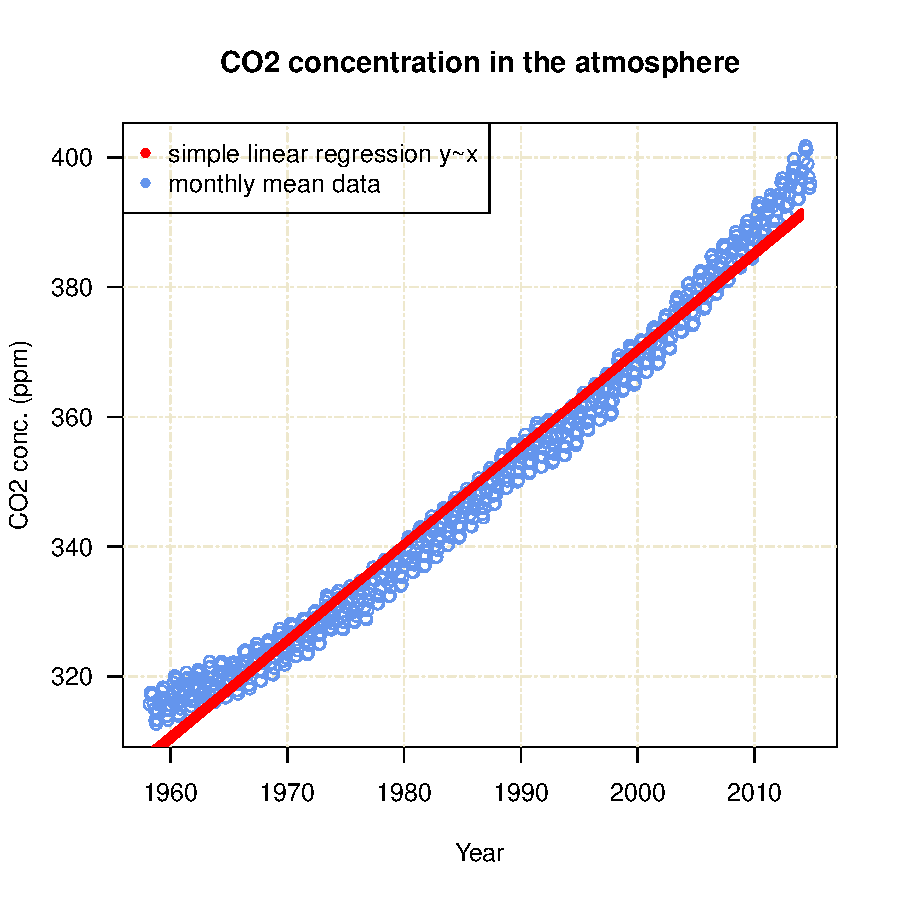
\includegraphics{FINAL_VERSION-plotorigin}
\caption{The raw data with a linear model}
\label{plotorigin}
\end{figure}

The plot 3 can be used to identify potential outliers in the dataset which could possibly bias the future model.  Due to the plot we can see, that we don't have any outliers and we can go on, having a look at the added simple poly-1 linear regression. The lm is not accurate in fitting the dataset. There are missing a lot of model predictors.

\begin{Schunk}
\begin{Sinput}
> xtable(summary(datalm)$coef, caption="Coefficients")
\end{Sinput}
% latex table generated in R 3.1.1 by xtable 1.7-4 package
% Fri Nov 28 19:10:44 2014
\begin{table}[ht]
\centering
\begin{tabular}{rrrrr}
  \hline
 & Estimate & Std. Error & t value & Pr($>$$|$t$|$) \\ 
  \hline
(Intercept) & -2618.56 & 16.98 & -154.23 & 0.00 \\ 
  year & 1.49 & 0.01 & 174.86 & 0.00 \\ 
   \hline
\end{tabular}
\caption{Coefficients} 
\end{table}\end{Schunk}
In the table 1, the standard errors of the linear regression are small.  One possible attribute of a time series is, that the residuals are serially correlated. With this autocorrelation, the standard errors shown in the lm would be underestimated, thus far too small.  Subsequently, the resulting significance  from the t-test (p-value) is lower than it should be. In our case this would mean, that CO2 concentrations are rising significantly and that we have a enormous problem with our atmospheric composition. 

\subsection{Dataset Transformation}
\noindent It is essential to transform your dataset into a timeseries (ts) if you seek for an accurate and extensive analysis of the data.
The data stored as a dataframe needs to be transformed with the important columns into the class of a time series to continue working on it properly. If you have monthly data you have to set the deltat of the function ts() to deltat=1/12 describing the sampling period parts between successive values xt and xt+1. Your time series should somehow look like table 1.\\
\noindent \textbf{Original Data}\\
\begin{Schunk}
\begin{Sinput}
> xtable(head(data), caption="Original CO2-Data")
\end{Sinput}
% latex table generated in R 3.1.1 by xtable 1.7-4 package
% Fri Nov 28 19:10:44 2014
\begin{table}[ht]
\centering
\begin{tabular}{rrr}
  \hline
 & year & co2 \\ 
  \hline
1 & 1958.21 & 315.71 \\ 
  2 & 1958.29 & 317.45 \\ 
  3 & 1958.38 & 317.50 \\ 
  4 & 1958.46 & 317.10 \\ 
  5 & 1958.54 & 315.86 \\ 
  6 & 1958.62 & 314.93 \\ 
   \hline
\end{tabular}
\caption{Original CO2-Data} 
\end{table}\end{Schunk}
\noindent \textbf{Transformation}\\
\begin{Schunk}
\begin{Sinput}
> yourts=ts(co2, c(1958,3),c(2014,10), deltat=1/12)
> class(yourts)
\end{Sinput}
[1] "ts"\begin{Sinput}
> time = time(yourts)
\end{Sinput}
\end{Schunk}

\subsection{Time-Series Visualization}%------------------------------------------------------------------------------------
It is  also helpful to get a quick overview of the time series class of our data with some plots.\\ 
The original data and the time series data are the same, however it is important to have a different class of \emph{ts} for further working on it. \\
\subsubsection{Time-Series Plot}
\begin{figure}[H]
\centering
\begin{Schunk}
\begin{Sinput}
> par(mfrow=c(1,1))
> plot(time, co2,type="n",las=1, xlab="Year", ylab="CO2 conc. (ppm)",
         main="CO2 concentration in the atmosphere")
> grid (NULL,NULL, lty = 6, col = "cornsilk2")
> points(yourts, col="cornflowerblue" )
> lines(year, co2, col="red")
> legend("topleft",c("time series", "monthly mean raw data"),
 pch=c(20,20), col=c("red", "cornflowerblue"))
\end{Sinput}
\end{Schunk}
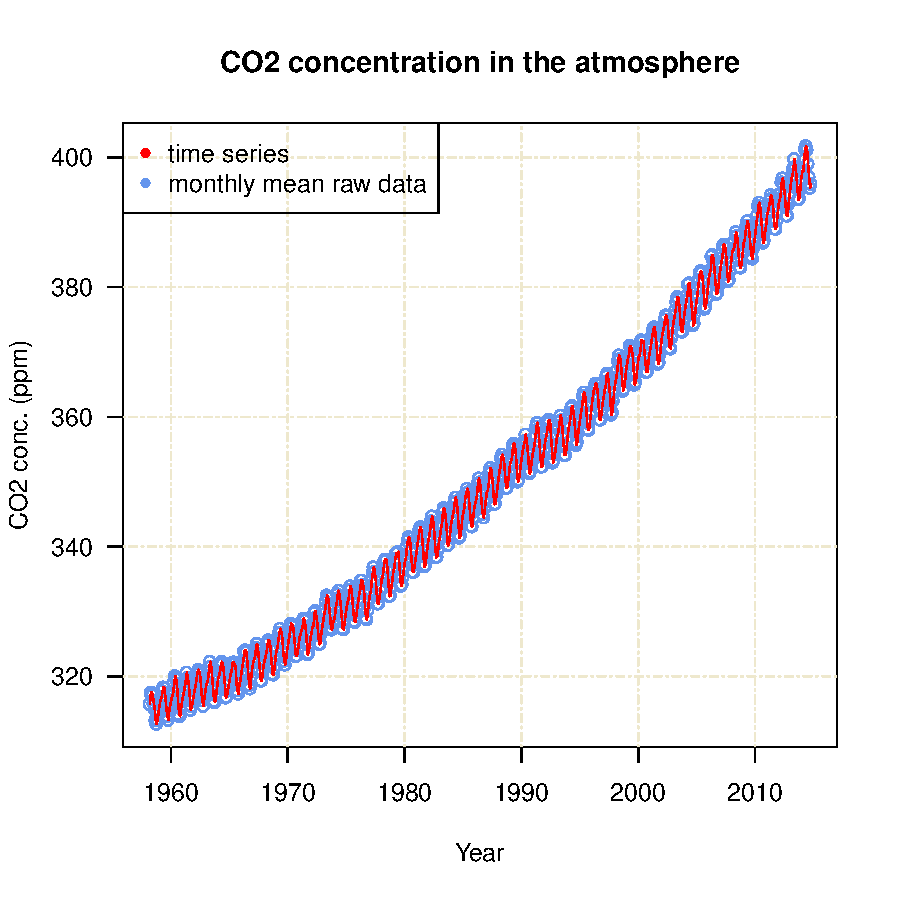
\includegraphics{FINAL_VERSION-fig1visualize}
\caption{Visualization of the CO2 Concentrations}
\label{fig1visualize}
\end{figure}

\subsubsection{ACF, PACF, SPECTRUM}

\noindent The correlogram is divided by three different functions all depicting important information on the autocorrelation and the cyclic component of our time series.  The problem we face with time series is the possible violation of independence assumption of a model, meaning that the SE is possibly too small. If the data are equally spaced in time,  the autocorrelation functions can be used to investigate residual  correlations in the model errors. The correlograms produce lags which are either within the CI or outter CI. If a lag is exceeding the CI, you need to include the lag as a order of autocorrelation in your AR or\- and MA terms which are needed in the following models. 


\begin{figure}[H]
 \begin{center}
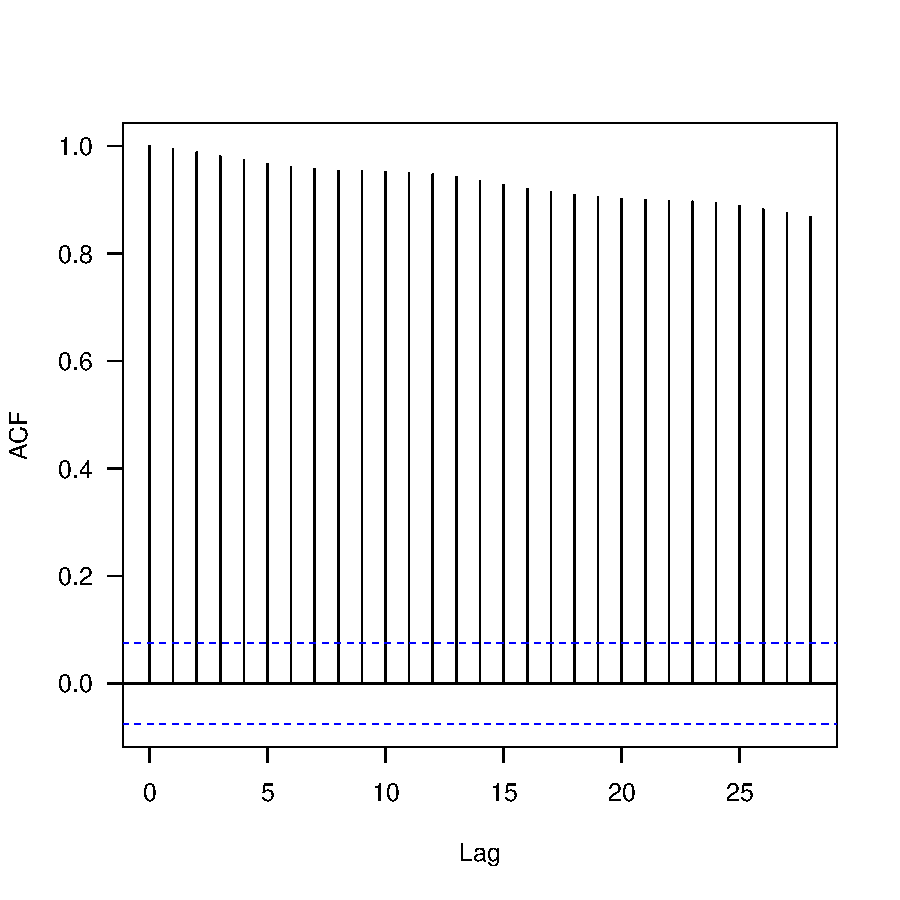
\includegraphics[width=0.5\textwidth]{FINAL_VERSION-correlogramlm.pdf}
 \caption{ACF of CO2 Concentrations with blue dotted lines as CI}
\label{correlogramlm}
\end{center}
\end{figure}

\noindent   \textbf{ACF}:  The autocorrelation function ACF() is one option producing a  plot of coefficients of correlation between your time series and lags of itself.   If you have a correlation at lag 1 and one at lag 2, the first correlation is reproduced to the second and so on to higher-order lags. This pattern, similar to the one in plot ~/ref{correlogramlm} is like a flow-on effect from the dependence at lag 1, which would be typical for an autoregressive process. \\
The \textbf{PACF (partial ACF)} is the accumulation of correlations between 2 variables excluding the correlation explained by their common correlation. It is not explained in the lower-order-lags. If you have correlations at lag 1 and at lag 2, the PACF computes the difference between the actual correlation at lag 2 and the expected correlation if reprdocution of the correlation at lag 1.  In our correlogram, the lag \emph{p=1}  included  as a autoregressive order in the model will capture already a lot of the correlation structure. \\
	The \textbf{spectrum} will be the third function used to check for possible correlation structures  showing the spectral density of the time series over frequencies. If a local maximum occurs,  \emph{1/(local max.)} can be used as equation to pick a possible periodic term. For our data we have a spectrum max at 0.75, meaning there might be a 12 * periodic cycle ( 12 months = 1 year) . \\

\begin{figure}[H]
\begin{center}
\subfloat[ACF]{
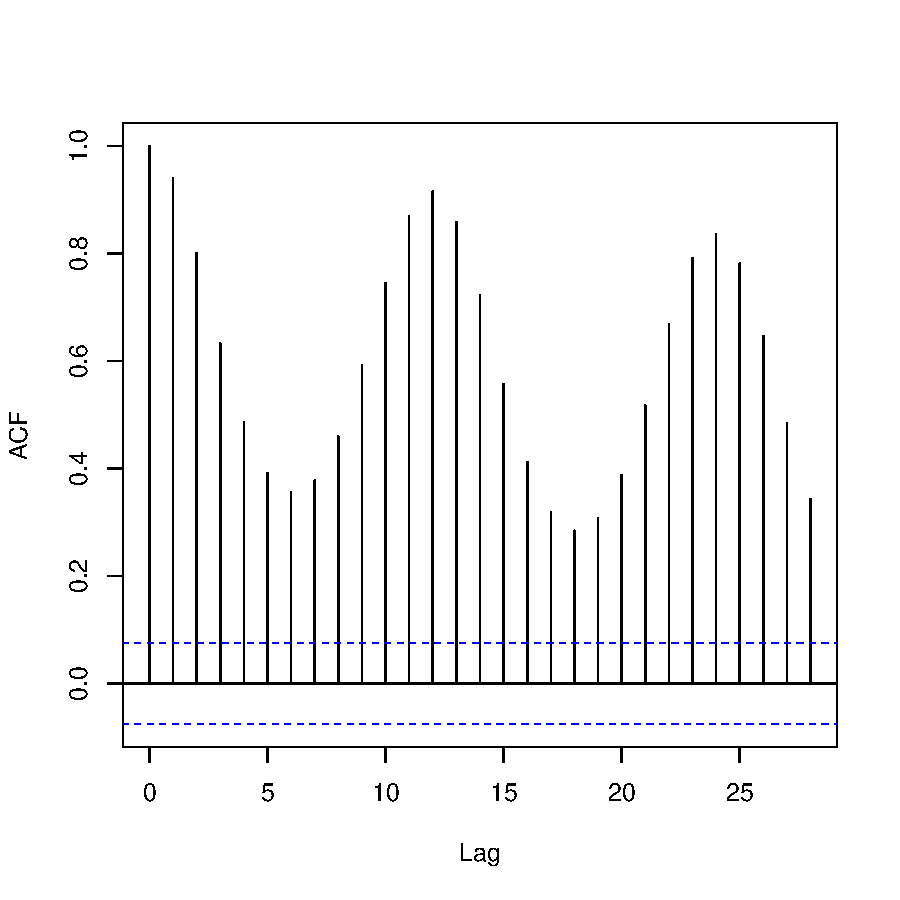
\includegraphics[width=0.4\textwidth]{FINAL_VERSION-correlogramres1.pdf}
}
\qquad
\subfloat[PACF]{
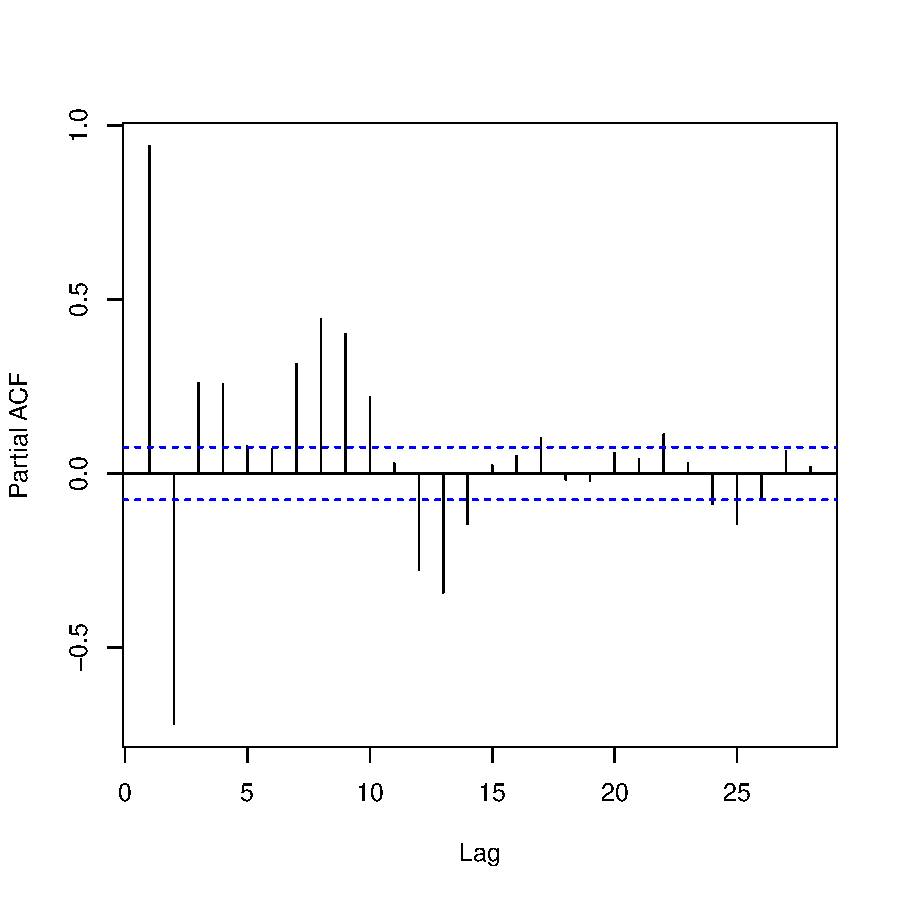
\includegraphics[width=0.4\textwidth]{FINAL_VERSION-correlogramres2.pdf}
}
\qquad
\subfloat[spectrum]{


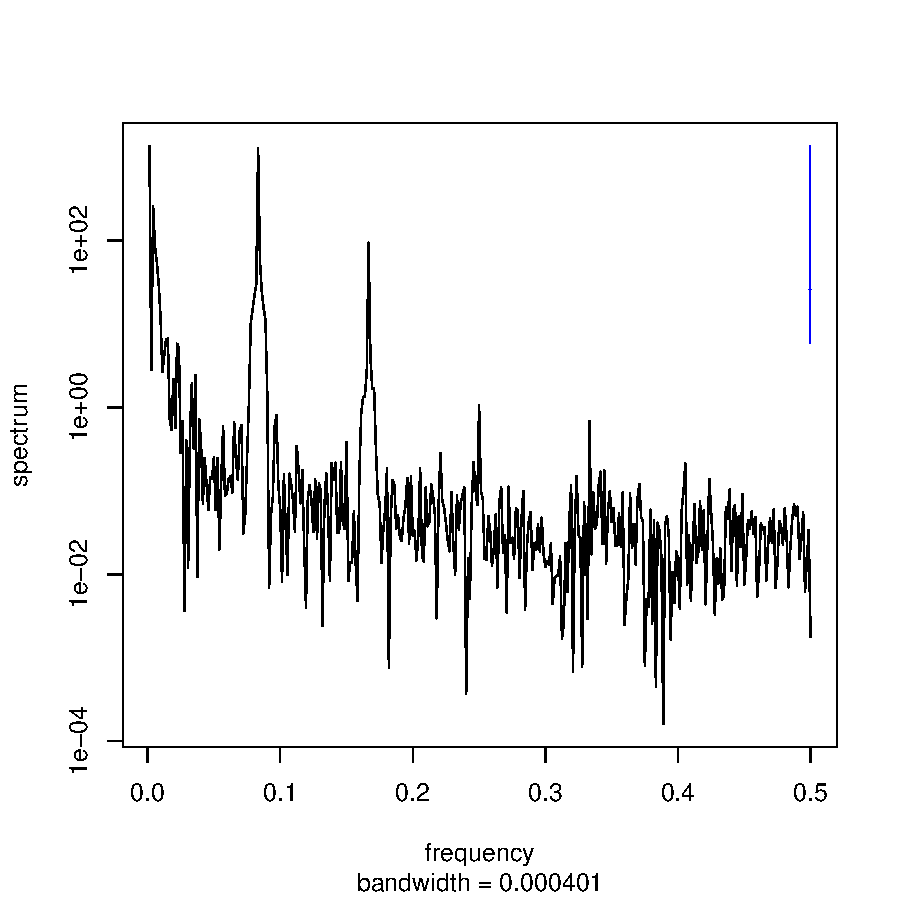
\includegraphics[width=0.4\textwidth]{FINAL_VERSION-correlogramres3.pdf}}
\end{center}
\caption{Correlogram of the residuals of datalm}
\label{corr_res_lm}
\end{figure}

\linebreak

\noindent	The residuals in a time series are serially correlated. The ACF is waving and decreases only slowly, which would be an identification of non-stationarity. We stop here all following diagnostic tests due to the clear autocorrelation in our data and investigate the different components of our time series. \\
  
  \pagebreak

\section{Decomposition of Time Series}%-----------------------------------------------------------------------------------------------------
As described in the Introduction, a time series consists usually of 3 components; a trend component, an irregular (random) component and (if it is a seasonal time series) a seasonal component. 

 
\subsection{Decomposing Seasonal Data}%----------------------------------------------------------------------------------------------------
\noindent We can decompose the ts and plot these components:


\begin{figure}[H]
\caption{Decomposition of the CO2 Time Series}
 \begin{center}
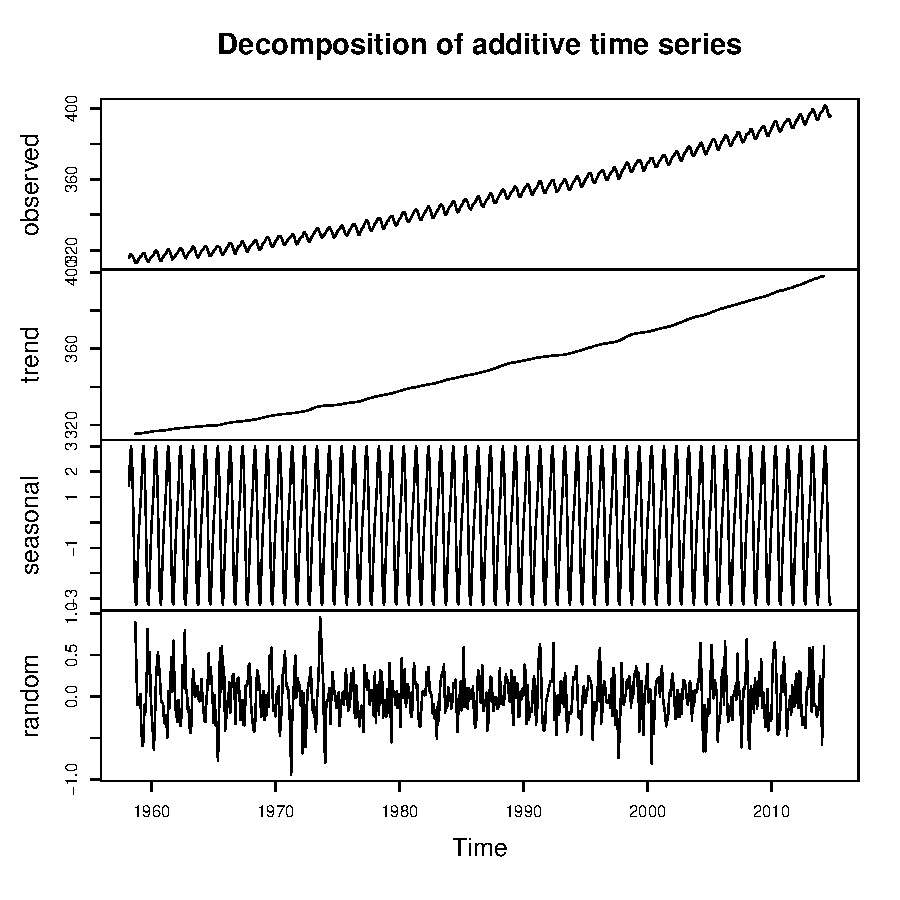
\includegraphics[width=0.5\textwidth]{FINAL_VERSION-decompose.pdf}
\label{decompose}
\end{center}
\end{figure}

\noindent We can see each component with:
\begin{Schunk}
\begin{Sinput}
> yourts_components<- decompose(yourts)
\end{Sinput}
\end{Schunk}
\begin{Schunk}
\begin{Sinput}
> yourts_components$seasonal
\end{Sinput}
\end{Schunk}


\begin{figure}[ht]
\begin{center}
\subfloat[monthly data]{
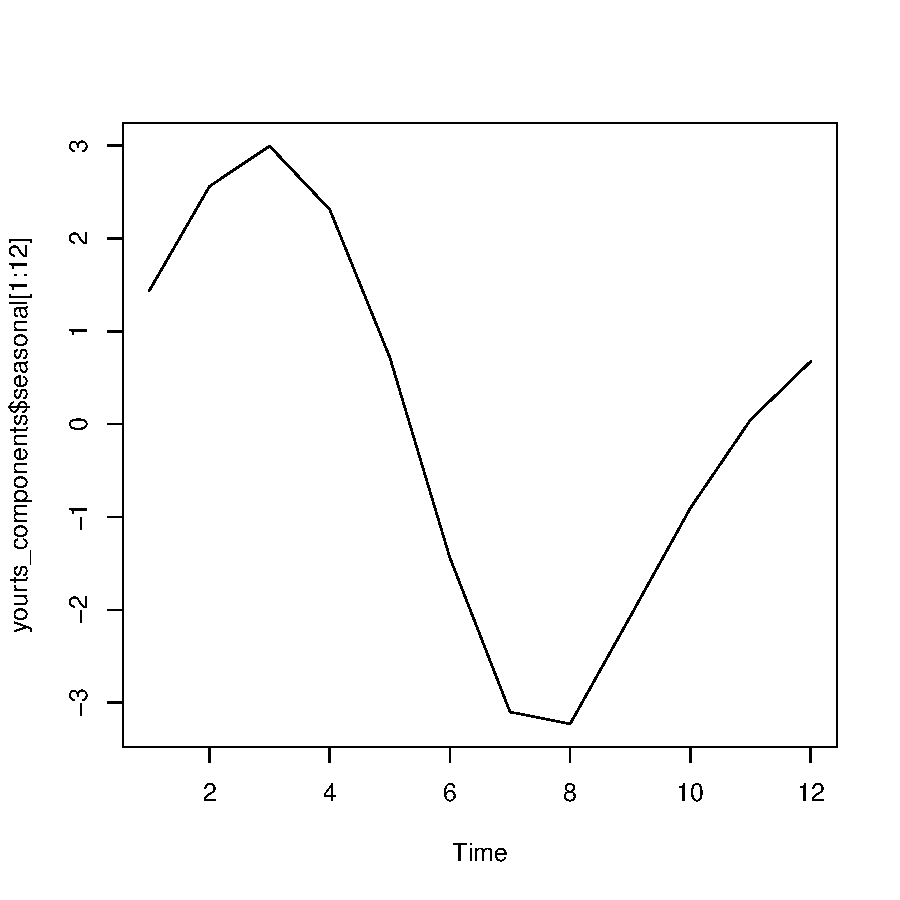
\includegraphics[width=0.4\textwidth]{FINAL_VERSION-seascomp1.pdf}
}
\qquad
\subfloat[annual]{
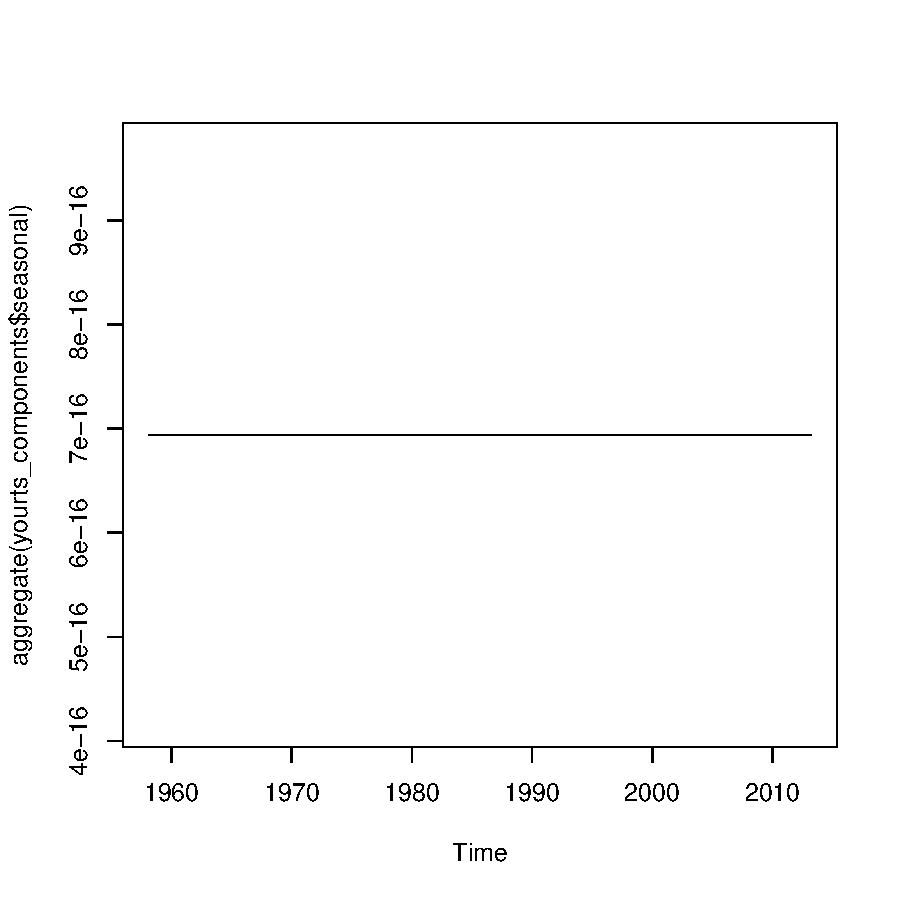
\includegraphics[width=0.4\textwidth]{FINAL_VERSION-seascomp2.pdf}
}
\end{center}
\caption{The seasonal component across the time}
\label{seascomp}
\end{figure}

In figure 8 , the monthly and annual component are depicted, respectively. It seems that our seasonal component is positive in the first half of the year ( month 1-6) and is negative in the second half of the year. The annual seasonal component is though constant within our time series. This assumes that we can fully include the seasonal term in an additive model without adding additional random noise to it or biasing the long-term trend. 

\begin{Schunk}
\begin{Sinput}
> yourts_seasonallyadjusted <- yourts - yourts_components$seasonal
\end{Sinput}
\end{Schunk}

\begin{figure}[ht]
\begin{center}
\subfloat[original]{
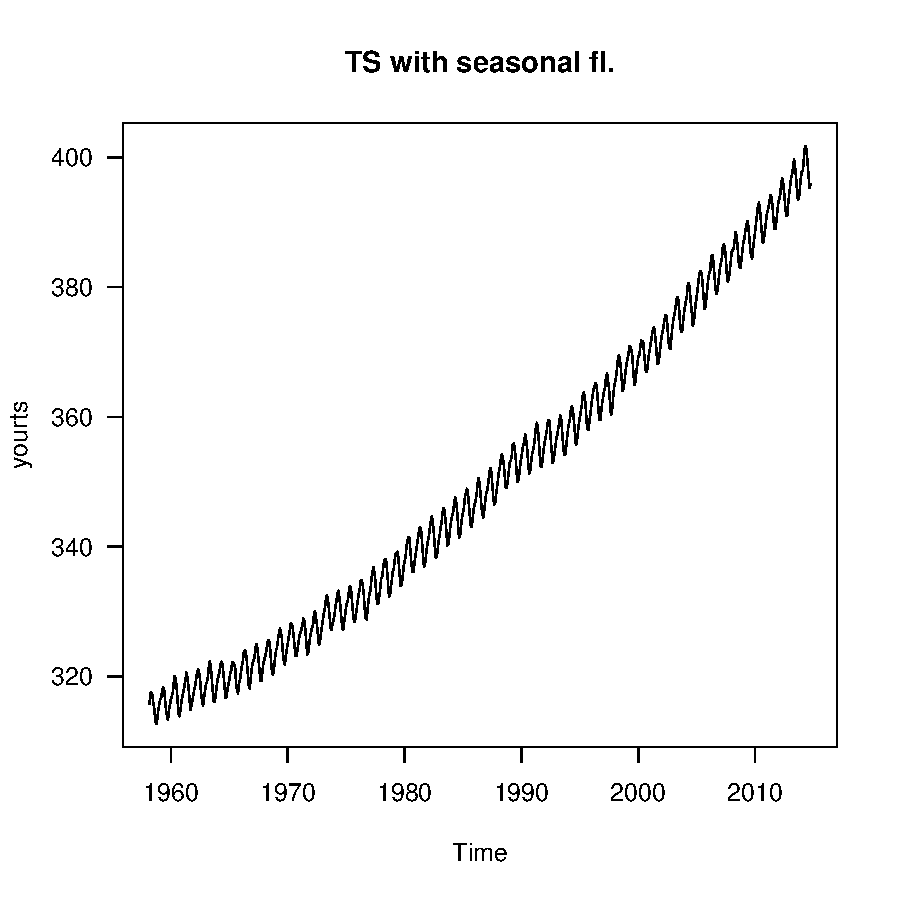
\includegraphics[width=0.4\textwidth]{FINAL_VERSION-seasadj1.pdf}
}
\qquad
\subfloat[seasadj.]{
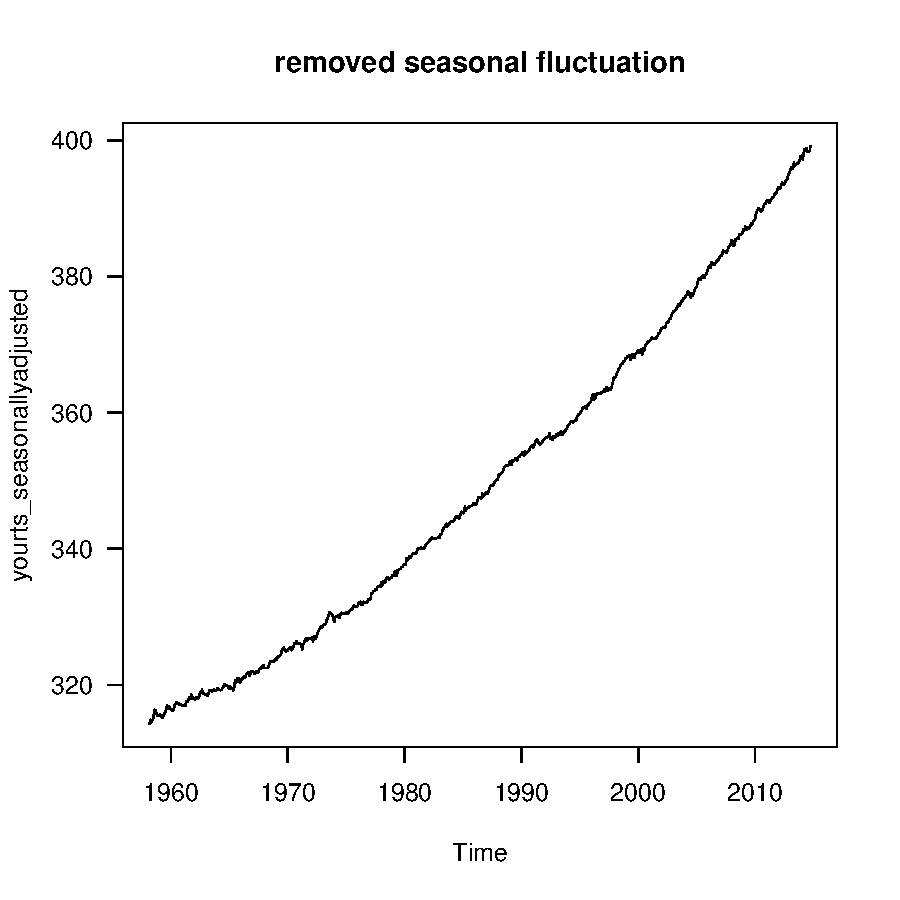
\includegraphics[width=0.4\textwidth]{FINAL_VERSION-seasadj2.pdf}
}
\end{center}
\caption{Comparison of seasonal vs. seasonally adjusted model}
\label{seasadj}
\end{figure}

\noindent Figure 9 depicts the comparison between the data with and without the seasonal fluctuation. In some cases it might be handy to have the model without the seasonal fluctuations to empahize the trend and the random part or to compute means more acurately.  


\section{Modelling the time series}
In this tutorial, the aim of the analysis of a seasonal time series is mainly  to generate forecasts  and make the time series stationary. For this, we need to define a model which has all the needed components of the time series. 

\begin{Schunk}
\begin{Sinput}
> adftable <- function(x) {
 stat.res =signif(adf.test(x)$p.value);
 stat.alt = adf.test(x)$alternative;
 c1 = cbind( stat.res, stat.alt);
 c2 = c("stationarity of time series",
         "alternative");
 matrixsmall = as.matrix(c1,c2);
 colnames(matrixsmall)= c("stationarity p-value",
         "alternative");
 return ( matrixsmall)
 }
\end{Sinput}
\end{Schunk}

After looking at the simple linear regression datalm, we were facing some serious problems with our model. To be sure about the stationarity we run an adf.test() giving p-value of 0.92, having a clear non-stationarity, what the future model needs to change. 

\begin{Schunk}
\begin{Sinput}
> xtable(adftable(yourts), main="Adf test for stationarity")
\end{Sinput}
\end{Schunk}

\begin{table}[ht]
\centering
\begin{tabular}{rll}
\hline
& stationarity p-value & alternative \\
\hline
1 & 0.928016 & stationary \\
\hline
\end{tabular}
\end{table}

Also we need a model, which is covering the serial correlation of our residuals. The ACF; PACF and the spectrum gives us certainty that there is some autocorrelation and seasonal fluctuation. glm() cannot allow for autocorrelation. The generalized least squares  model is one option that can be used to allow for autocorrelation of standard errors and unequal variances. 


\subsection{Analysis of Seasonal Data with GLS}

The generalized least squares  model is one option that can be used to allow for autocorrelation of standard errors and unequal variances. In the gls() we have different options to choose for our covariance structure. Because our data is not spatially correlated we are not discussing spatial autocorrelation here.\\

For temporal correlation we have five options:
\begin{enumerate}
\item corAR1: in ACF exponential decreasing values of correlation with time distance\\
\item corARMA: either autoregressive order or moving average order or both\\
\item corCAR1: continuous time ( time index does nto have to be integers)\\
\item corCompSymm: correlation does not decrease with higher distance\\
\item corSymm: general correlation only for few observations only, often overparameterized\\
\end{enumerate}



Our first gls() model accounts for the AR1, which is clearly visible in the PACF. 
Our lag 1 is the lag computed from the linear regression ACF.

\begin{Schunk}
\begin{Sinput}
> data.glsAR = gls(yourts ~ time,cor= corAR1(acf(resid(datalm))$acf[2]))
> save(data.glsAR, file="data.glsAR.RData")
\end{Sinput}
\end{Schunk}

\begin{Schunk}
\begin{Sinput}
> load("data.glsAR.RData")
\end{Sinput}
\end{Schunk}


\begin{figure}[ht]
\begin{center}
\subfloat[original]{
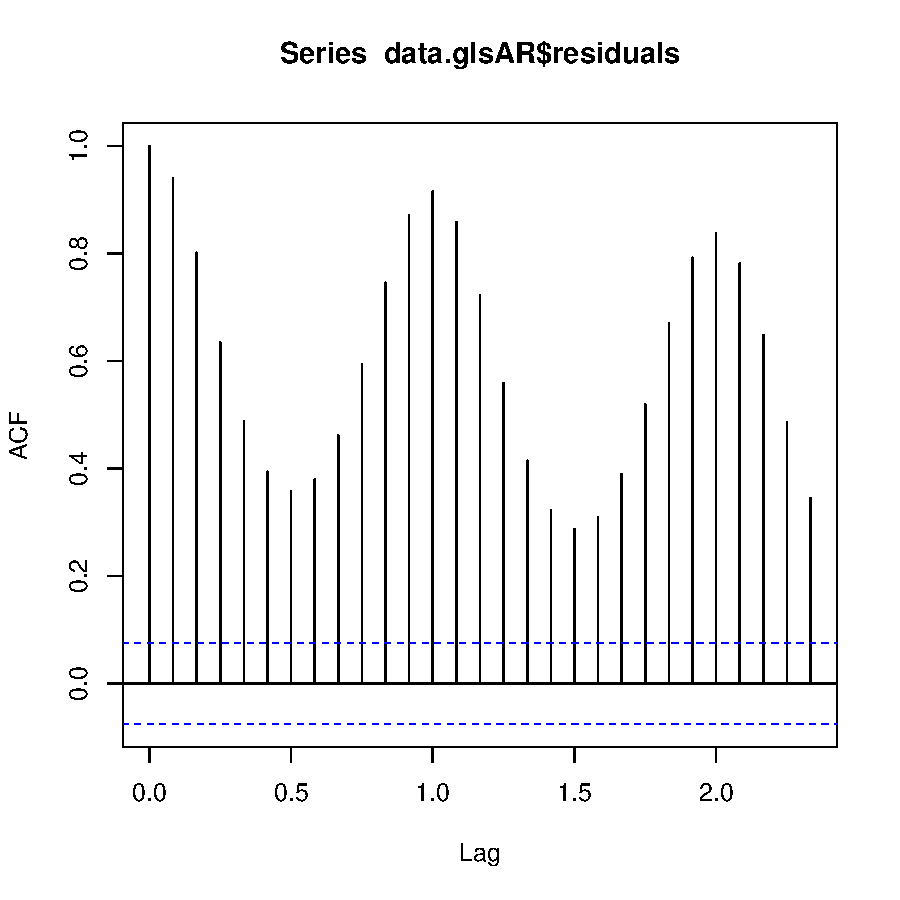
\includegraphics[width=0.4\textwidth]{FINAL_VERSION-glsARACF.pdf}
}
\qquad
\subfloat[seasadj.]{
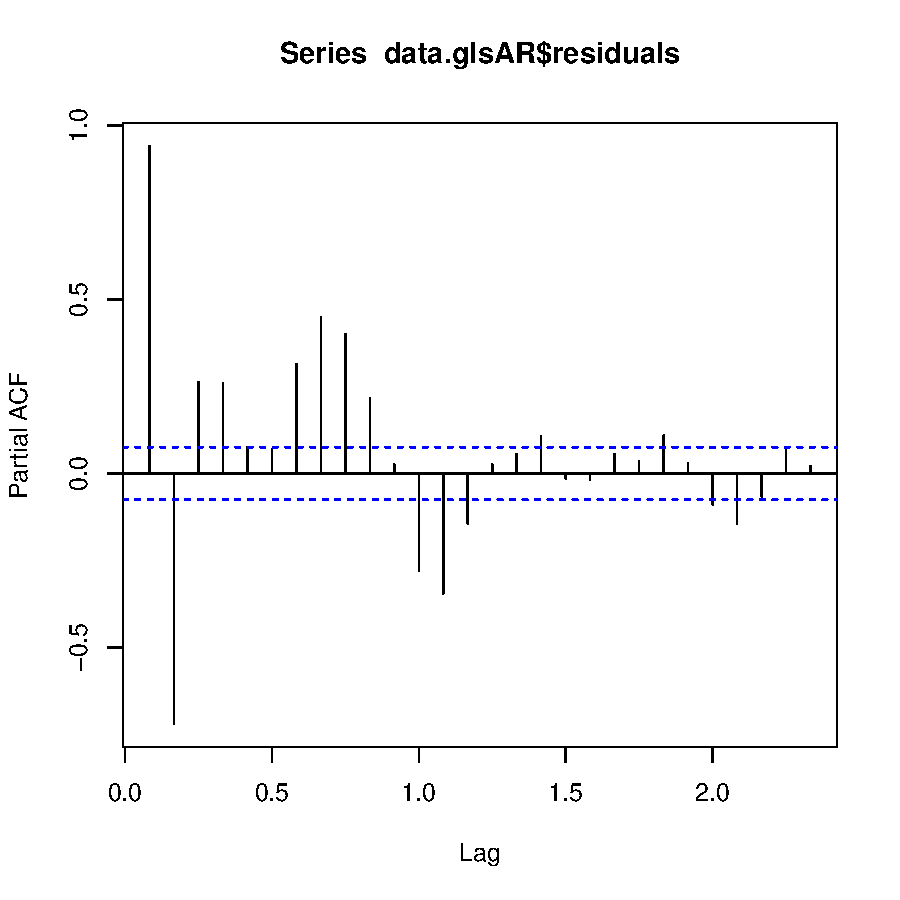
\includegraphics[width=0.4\textwidth]{FINAL_VERSION-glsARPACF.pdf}
}
\end{center}
\caption{Correlogram of GLS  with AR(1) structure}
\label{corglsAR}
\end{figure}


We still face a lot of problems with the first GLS model only including 1 auto regressive order. 
One option is to allow the AR to use more parameters and/or to include a moving average or error variance to the model. This can be handled via the corARMA. We tried 2 versions, one with 1 lag and 1 moving average, the other with 2 lags and 2 moving averages.
The 0.2 are starting values for Phi, which are in the modelling process optimized.
The next models are thus:
\begin{Schunk}
\begin{Sinput}
> dataglsARMA10 = gls ( yourts ~ time, cor = corARMA (p=1, q=0 ))
> dataglsARMA11 = update (dataglsARMA10, cor=corARMA(p=1, q=1))
> dataglsARMA12 = update (dataglsARMA10, cor=corARMA(p=1, q=2))
> dataglsARMA22 = update (dataglsARMA10, cor=corARMA(p=2, q=2))
> dataglsARMA21 = update (dataglsARMA10, cor=corARMA(p=2, q=1))
> save(dataglsARMA10, file="dataglsARMA10.RData")
> save(dataglsARMA11, file="dataglsARMA11.RData")
> save(dataglsARMA12, file="dataglsARMA12.RData")
> save(dataglsARMA22, file="dataglsARMA22.RData")
> save(dataglsARMA21, file="dataglsARMA21.RData")
> 
\end{Sinput}
\end{Schunk}

\begin{Schunk}
\begin{Sinput}
> load(file="dataglsARMA10.RData")
> load( file="dataglsARMA11.RData")
> load( file="dataglsARMA12.RData")
> load( file="dataglsARMA22.RData")
> load( file="dataglsARMA21.RData")
\end{Sinput}
\end{Schunk}

The AIC (Akaike Information Criterion) is used to compare the different models. The smaller the AIC value, the better fits the model to the original dataset.  
To compare all the models we use anova and the best model is so far the dataglsARMA22 with the lowest AIC and significantly better than the ARMA(2,1), which is itself not better than the ARMA(1,2), but this is better than the previous 2 models. 

\begin{Schunk}
\begin{Sinput}
> anova(dataglsARMA10,dataglsARMA11,dataglsARMA12,dataglsARMA21,dataglsARMA22)
\end{Sinput}
\begin{Soutput}
              Model df      AIC      BIC     logLik   Test
dataglsARMA10     1  4 2189.575 2207.651 -1090.7874       
dataglsARMA11     2  5 1760.113 1782.709  -875.0567 1 vs 2
dataglsARMA12     3  6 1587.709 1614.824  -787.8545 2 vs 3
dataglsARMA21     4  6 1549.076 1576.191  -768.5380       
dataglsARMA22     5  7 1495.348 1526.982  -740.6742 4 vs 5
               L.Ratio p-value
dataglsARMA10                 
dataglsARMA11 431.4614  <.0001
dataglsARMA12 174.4045  <.0001
dataglsARMA21                 
dataglsARMA22  55.7275  <.0001
\end{Soutput}
\end{Schunk}

\begin{Schunk}
\begin{Sinput}
> diagnostics(dataglsARMA22)
\end{Sinput}
\begin{Soutput}
     normality    stat.res   stat.res.alt
[1,] "1.8632e-08" "0.928016" "stationary"
     autocorr            indep
[1,] "0.111186713062342" "0"  
\end{Soutput}
\end{Schunk}



\begin{figure}[ht]
\begin{center}
\subfloat[residuals]{
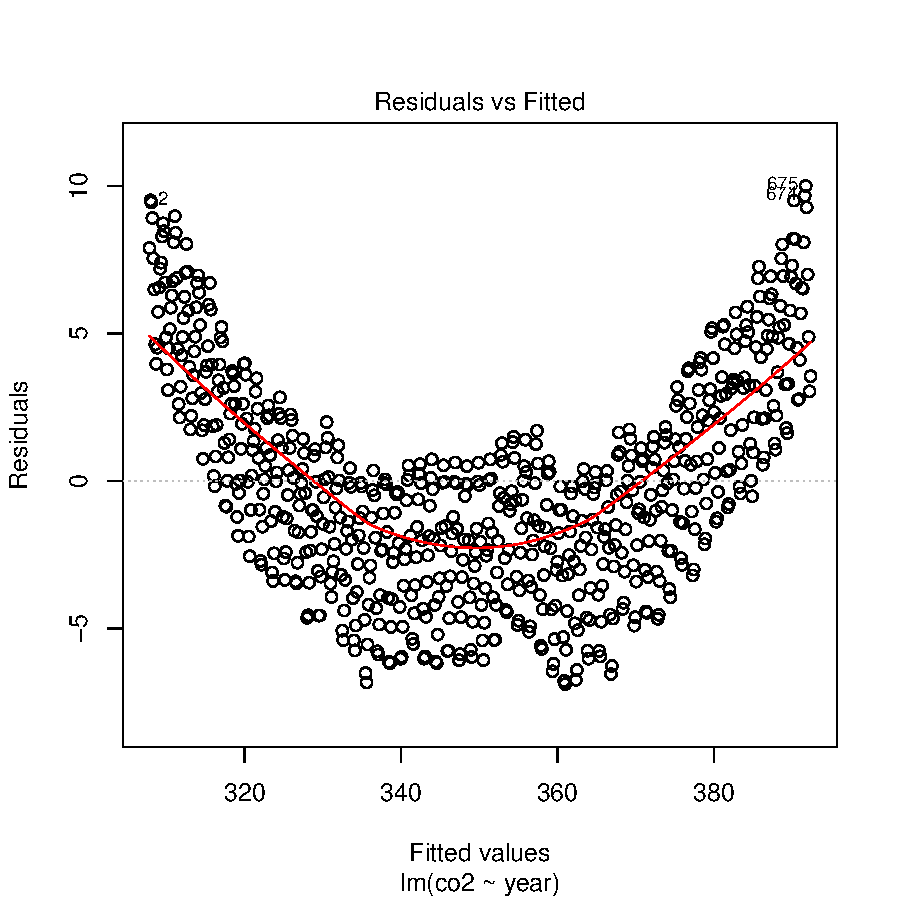
\includegraphics[width=0.4\textwidth]{FINAL_VERSION-residual.pdf}
}
\qquad
\subfloat[seasadj.]{
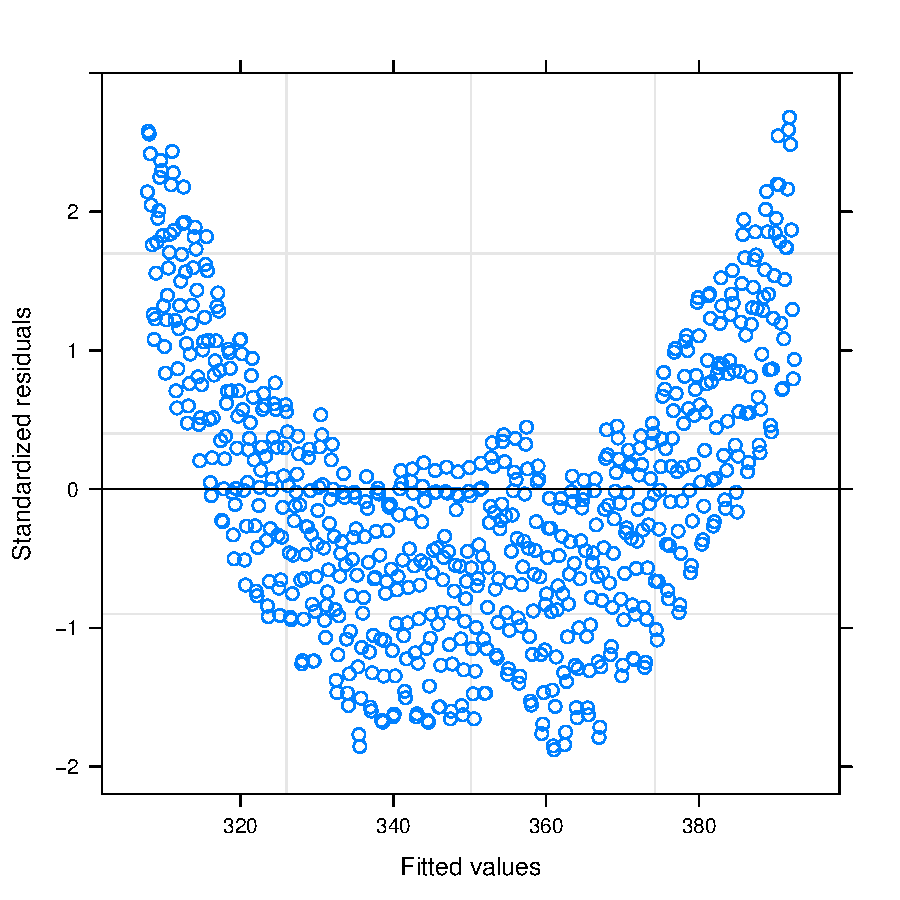
\includegraphics[width=0.4\textwidth]{FINAL_VERSION-residualARMA.pdf}
}
\end{center}
\caption{Residuals fitted vs. observed in (a) LM and (b) GLS}
\label{residual}
\end{figure}

\noindent Now, the best correlation structure seems to be selected, however the seasonal component is still missing. We need to include that in a simple version: 


\begin{Schunk}
\begin{Sinput}
> seas = cycle(yourts)
> dataseasongls = gls(yourts ~ time + factor(seas),
                     cor=corARMA(c(0.2,0.2,0.2,0.2),
                                 p=2, q=2))
> save(dataseasongls, file="dataseasongls.RData")
\end{Sinput}
\end{Schunk}

\begin{Schunk}
\begin{Sinput}
> load("dataseasongls.RData")
\end{Sinput}
\end{Schunk}

\begin{figure}[ht]
\begin{center}
\subfloat[ACF]{
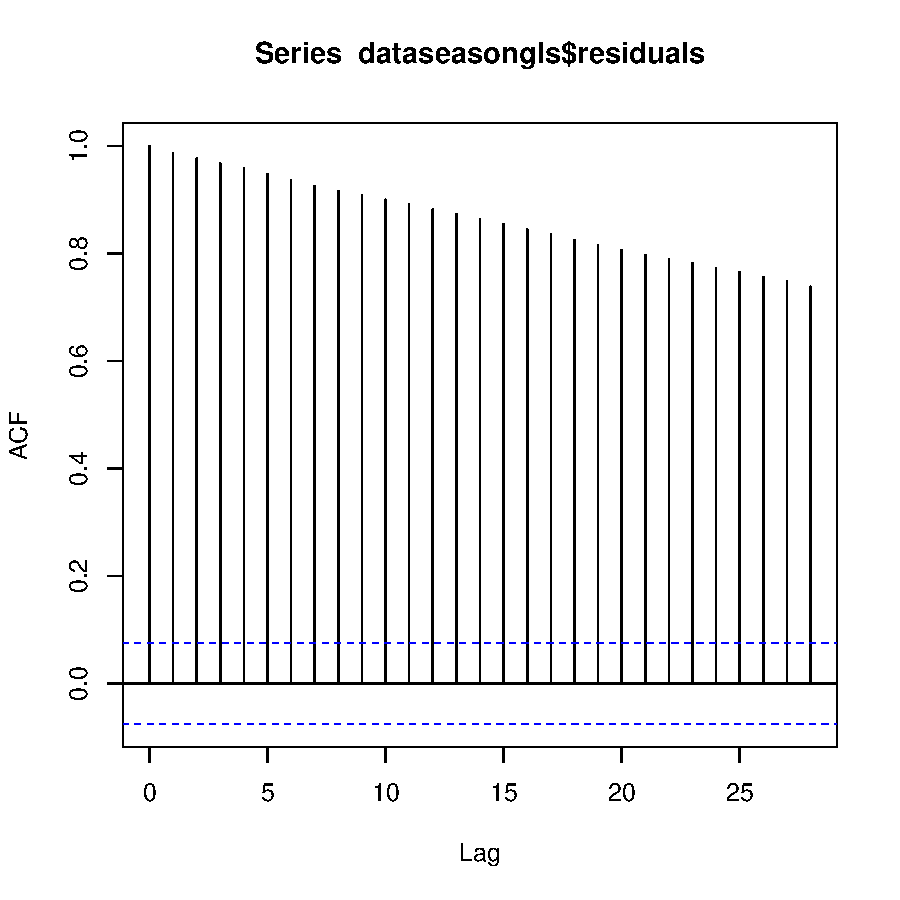
\includegraphics[width=0.4\textwidth]{FINAL_VERSION-corseas1.pdf}
}
\qquad
\subfloat[PACF]{
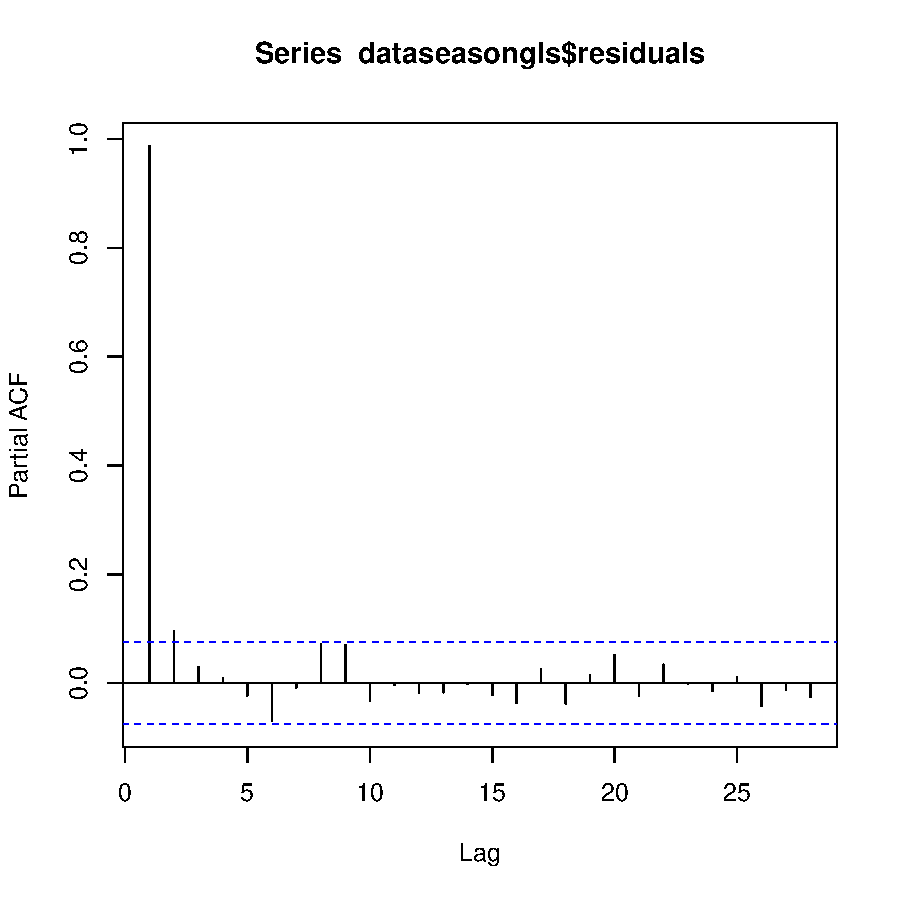
\includegraphics[width=0.4\textwidth]{FINAL_VERSION-corseas2.pdf}
}
\end{center}
\caption{Correlogram of seasonality-including model}
\label{corseas}
\end{figure}

\begin{Schunk}
\begin{Sinput}
> par(mfrow=c(1,1))
> plot(dataseasongls$residuals,ylab="Residuals", xlab="Year", 
      las=1, type="p", col="cornflowerblue", 
      main="Residuals of dataseasongls over time") 
\end{Sinput}
\end{Schunk}

\begin{figure}[H]
 \begin{center}
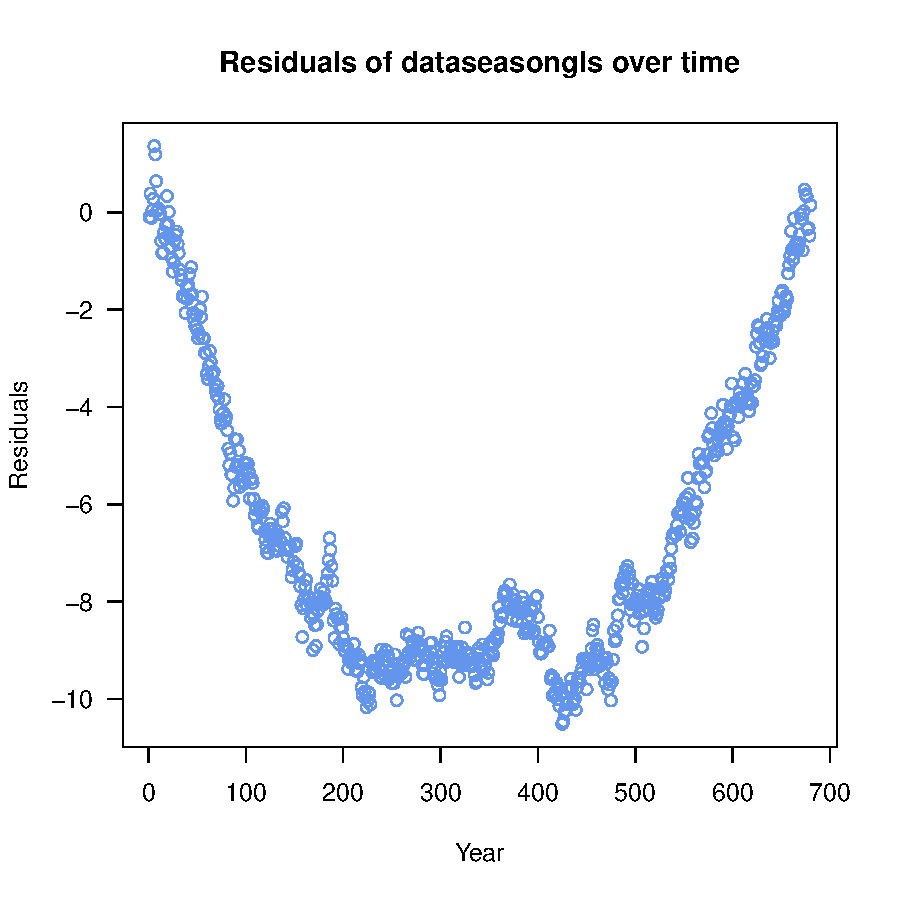
\includegraphics[width=0.4\textwidth]{FINAL_VERSION-resseas.pdf}
\caption{Residuals of seasonality-including model}
\label{resseas}
\end{center}
\end{figure}

The problem with anova.gls is that it cannot compare gls() with different fixed effects. The added seasonal term is such an effect, thus the anova does not work here. We need to compare the AIC by hand and see an improvement. 


\begin{Schunk}
\begin{Sinput}
> AIC(dataglsARMA22)
\end{Sinput}
[1] 1495.348\begin{Sinput}
> AIC(dataseasongls)
\end{Sinput}
[1] 401.2934\end{Schunk}

\begin{figure}[H]
\centering
\begin{Schunk}
\begin{Sinput}
> ts.plot(cbind(yourts, dataglsARMA22$fitted,
               dataseasongls$fitted),
         lty=1:2, col=c(1,2,3), 
         main="Compare mean monthly data with gls model")
> legend(1960,400,c("Original",
                   "Fitted for Autocorrelation",
                   "Fitted for Seasonality"),
        col=c(1,2,3),lty=c(1, 2,3))
\end{Sinput}
\end{Schunk}
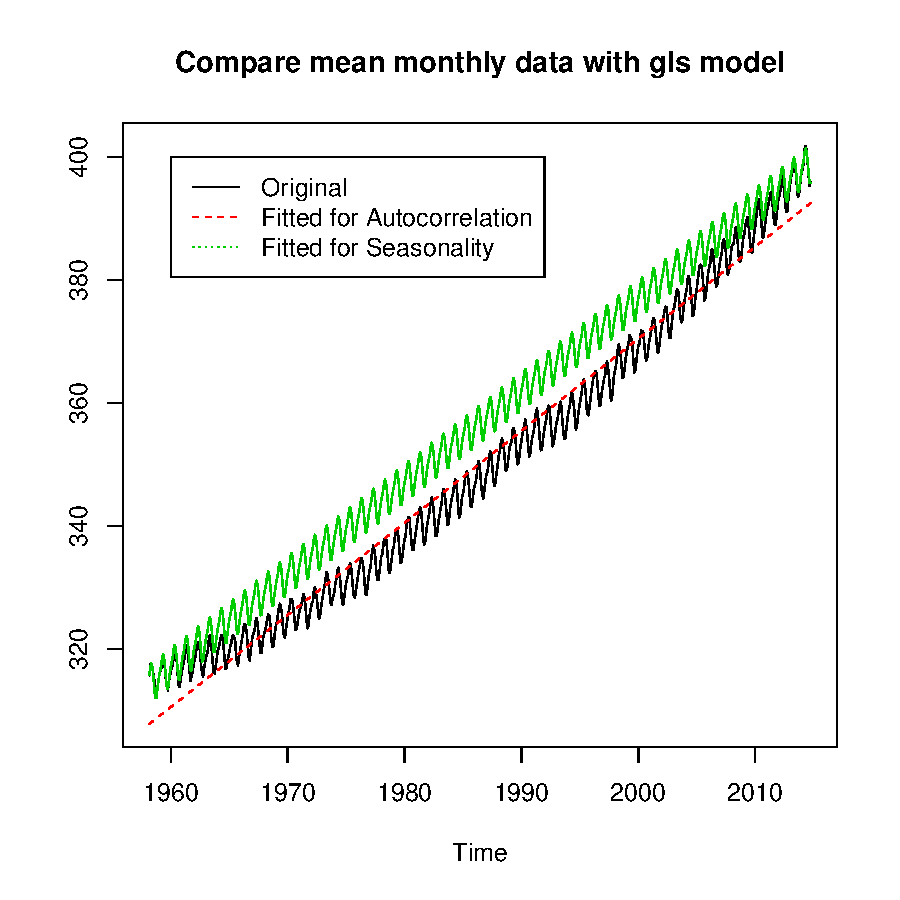
\includegraphics{FINAL_VERSION-045}
\caption{Comparison of seasonality-including model with only autocorrelation-including model}
\label{compseas2}
\end{figure}

In the figure ~\ref{compseas2} you see the options we were trying so far to come closer to our adequate model. One option is the ARMA22 GLS including autocorrelation, the second option is to include the seasonality by adding a fixed effect (factor(season)) to our gls. 
The seasonal effect inclusion clearly improves our model. But the original data is slightly curved and we see in plot ~/ref{resseas} that the residuals get bigger as soon as the bending of the original data sets in and flatten again as soon as the model was close to the end point in 2014. \\

We should include a quadratic term and generalize our seasonality with a continuous sin-cos wave:\\

\begin{Schunk}
\begin{Sinput}
> SIN = COS = matrix(nr=length(yourts), nc=6)
> for (i in 1:6) {
   COS[,i] <- cos(2*pi*i*time(yourts))
   SIN[,i] <- sin(2*pi*i*time(yourts)) 
 }
> time = time(yourts)
\end{Sinput}
\end{Schunk}
#also was done by hand in self writing seasonality removal above
Thus we do not know how many changes in the wave we need to include, we include 6 changes in the wave to be certain that the next model can follow the best wave option. 

Before this, add a quadratic term ( polynomial (x,2)), x = years) will change the linear regression by including a slight bending in the fitted values over time, which we saw in the original data. 


\begin{Schunk}
\begin{Sinput}
> harmonizedgls<-gls(yourts ~ time + I(time^2) +
                     COS[,1]+SIN[,1]+COS[,2]+SIN[,2]+
                     COS[,3]+SIN[,3]+COS[,4]+SIN[,4]+
                     COS[,5]+SIN[,5]+COS[,6]+SIN[,6],
                   corr=corAR1(acf(dataseasongls$residuals)$acf[2]))
> save(harmonizedgls, file="harmonizedgls.RData")
> harmonizedARMAgls<-gls(yourts ~ time + I(time^2) +
                       COS[,1]+SIN[,1]+COS[,2]+SIN[,2]+
                       COS[,3]+SIN[,3]+COS[,4]+SIN[,4]+
                       COS[,5]+SIN[,5]+COS[,6]+SIN[,6]
                     , cor=corARMA(p=2, q=2))
> save(harmonizedARMAgls, file="harmonizedARMAgls.RData")
\end{Sinput}
\end{Schunk}

\begin{Schunk}
\begin{Sinput}
> load("harmonizedARMAgls.RData")
> load("harmonizedgls.RData")
\end{Sinput}
\end{Schunk}

\begin{Schunk}
\begin{Sinput}
> AIC(harmonizedgls) #even smaller 
\end{Sinput}
\begin{Soutput}
[1] 396.86
\end{Soutput}
\begin{Sinput}
> AIC(harmonizedARMAgls) #even smaller 
\end{Sinput}
\begin{Soutput}
[1] 360.4082
\end{Soutput}
\begin{Sinput}
> #(anova(harmonizedgls,harmonizedARMAgls))
\end{Sinput}
\end{Schunk}

\begin{table}[H]
\centering
\begin{tabular}{rlrrrrrlrr}
\hline
&  & Model & df & AIC & BIC & logLik & Test & L.Ratio & p-value \\
\hline
&harmonizedgls  & 1 & 17 & 396.86 & 473.36 & -181.43 & & & \\
&harmonizedARMAgls  & 2 & 20 & 360.41 & 450.40 & -160.20 & 1 vs 2 & 42.45 & 0.00 \\
\hline
\end{tabular}
\end{table}

\begin{figure}[H]
\centering
\begin{Schunk}
\begin{Sinput}
> par(mfrow=c(1,1))
> ts.plot(cbind(yourts,dataseasongls$fitted, harmonizedARMAgls$fitted),
         col=c(1,2,3),
         main="Compare mean monthly data with gls model")
> legend(1960,400,c("Original", "Included seasonality ",
                   "Polynm. + seasonality"),
         col=c(1,2,3), pch=c(20,20,20))
\end{Sinput}
\end{Schunk}
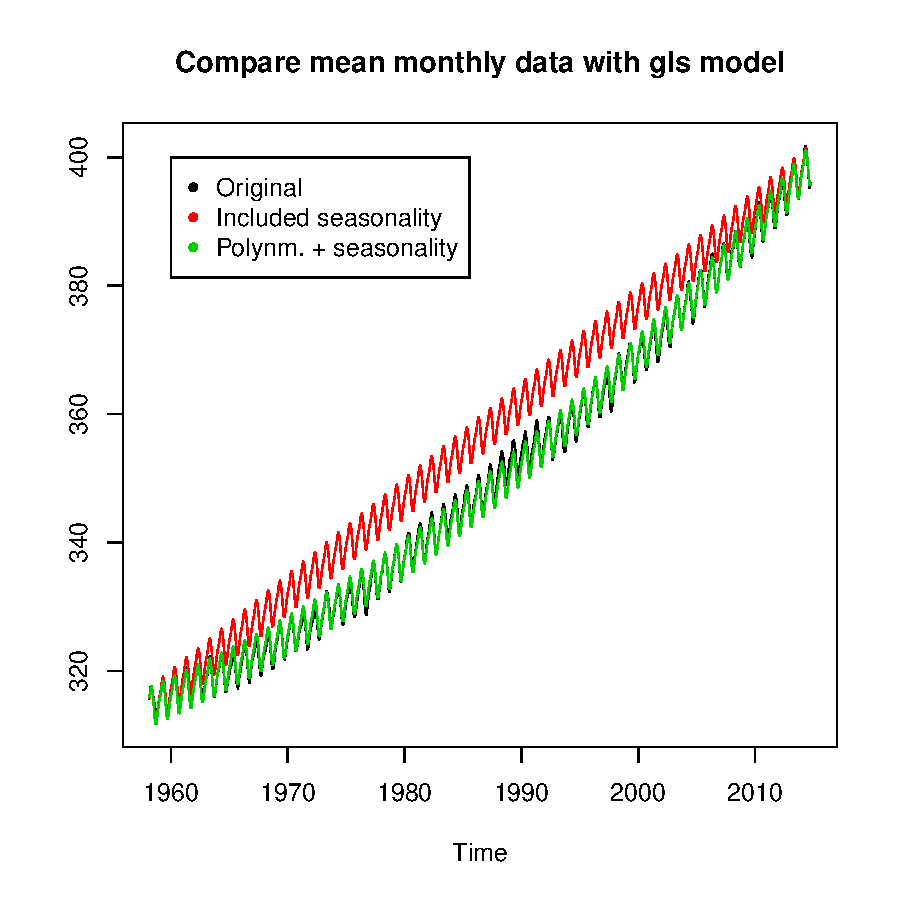
\includegraphics{FINAL_VERSION-050}
\caption{Comparison of season and quadr. term included model}
\label{compq}
\end{figure}

\linebreak
In Figure 15 we were plotting our different approaches with the best AIC together and can see a significant improvement in the fit of the harmonized gls() which was including a quadratic term and the seasonality. \\

\begin{figure}[ht]
\begin{center}
\subfloat[LM]{
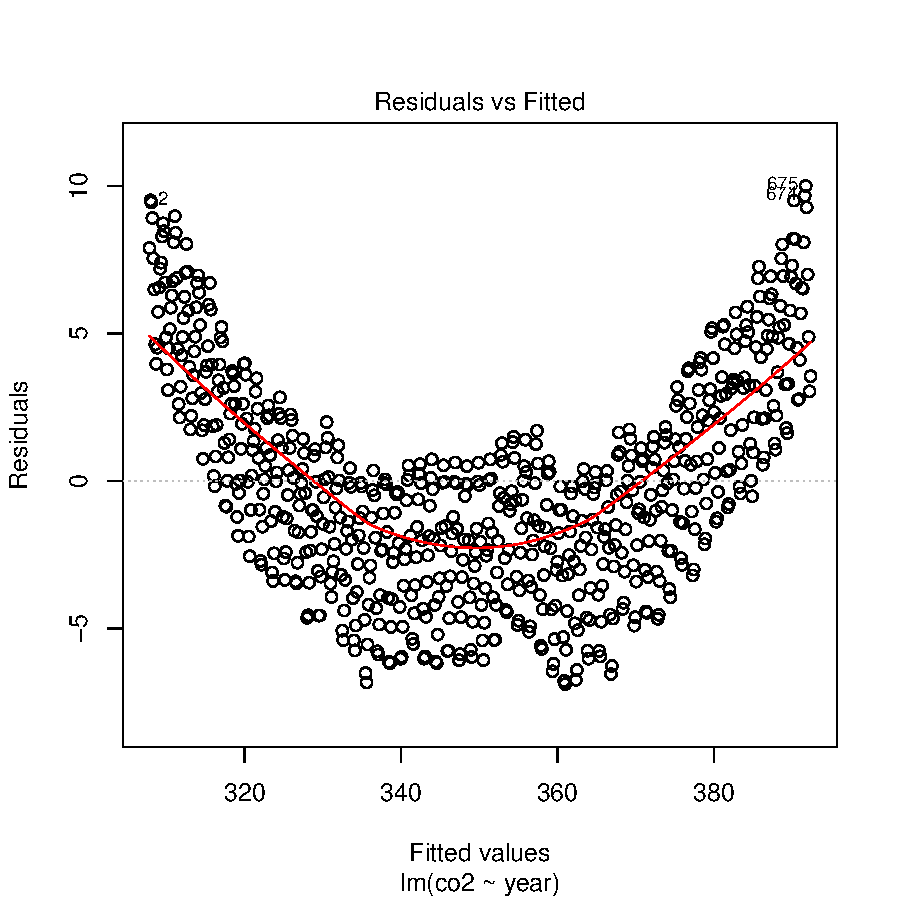
\includegraphics[width=0.45\textwidth]{FINAL_VERSION-comparison_finalgls1.pdf}
}
\qquad
\subfloat[ARMA]{
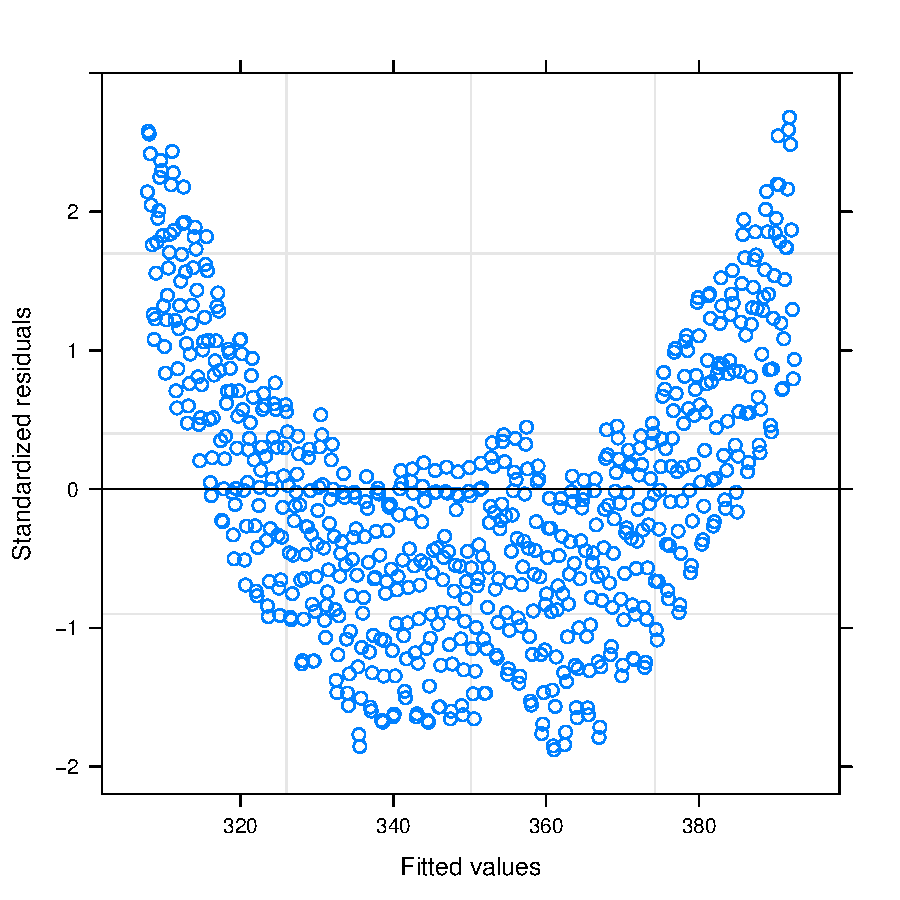
\includegraphics[width=0.4\textwidth]{FINAL_VERSION-comparison_finalgls2.pdf}
}
\qquad
\subfloat[quadrARMA]{
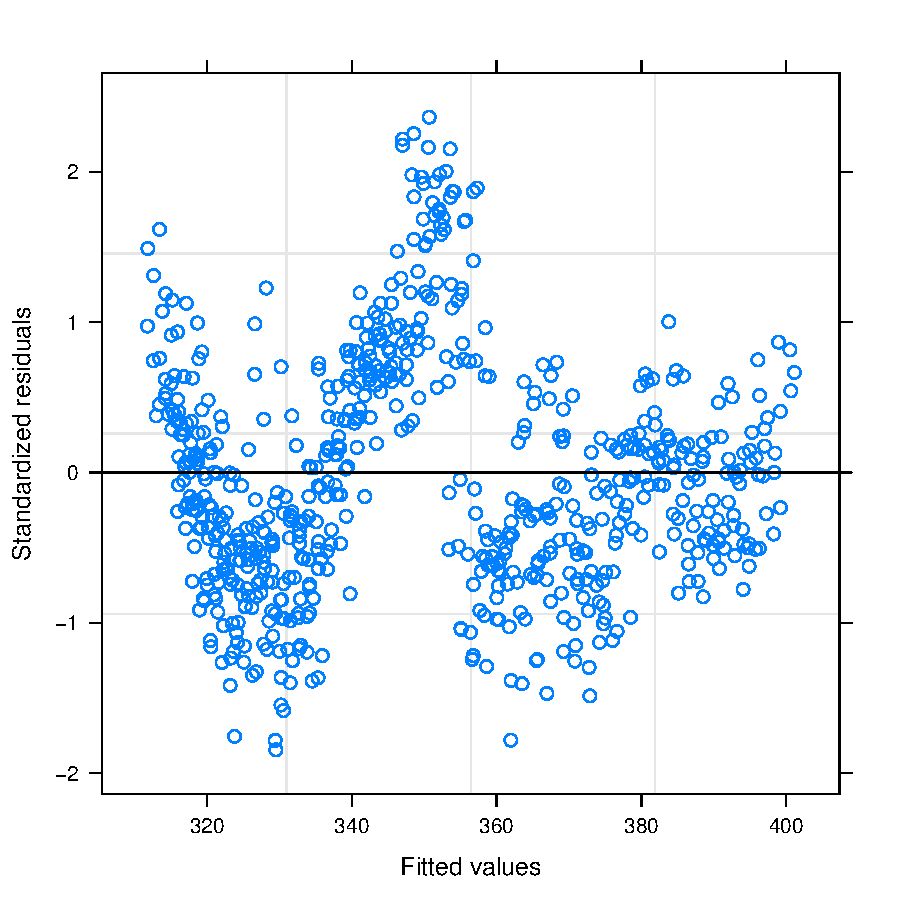
\includegraphics[width=0.4\textwidth]{FINAL_VERSION-comparison_finalgls3.pdf}
}
\end{center}
\caption{Comparison of residuals vs. fitted values for lm, gls/arma, and the quadratic gls/arma}
\label{comparison_finalgls}
\end{figure}

\begin{Schunk}
\begin{Sinput}
> diagnostics(harmonizedARMAgls)
\end{Sinput}
\begin{Soutput}
     normality     stat.res   stat.res.alt
[1,] "5.22872e-08" "0.290355" "stationary"
     autocorr           indep
[1,] "0.18333304071156" "0"  
\end{Soutput}
\end{Schunk}




\begin{figure}[H]
\begin{center}
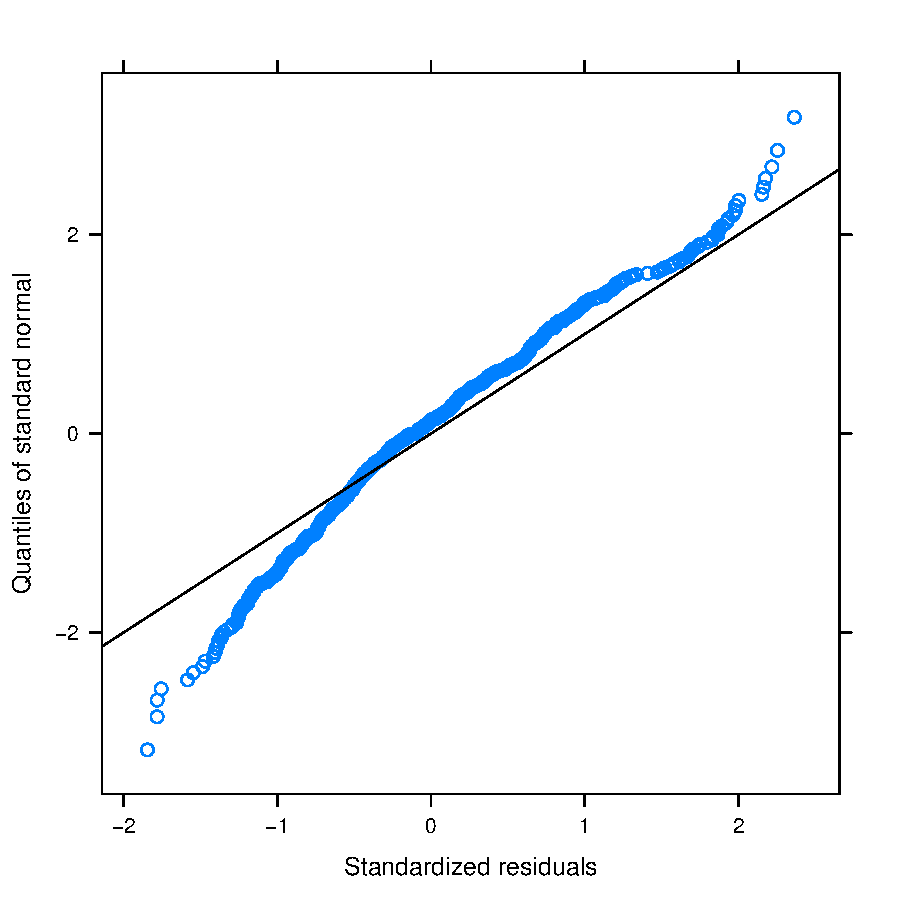
\includegraphics[width=0.5\textwidth]{FINAL_VERSION-finalgls_norm.pdf}
\caption{look at norm. distribution}
\label{finalgls_norm}
\end{center}
\end{figure}

\linebreak
#bestmodel with smallest AIC: \\
\begin{Schunk}
\begin{Sinput}
> anova.all = anova( harmonizedgls,harmonizedARMAgls)
> #as.matrix(anova.all)
> bestmodel= anova.all$Model[anova.all$AIC ==min(anova.all$AIC)]
> bestmodel 
\end{Sinput}
\begin{Soutput}
[1] 2
\end{Soutput}
\end{Schunk}


\linebreak

In the beginning we were talking about the underestimation of standard errors in the linear model, if not considering the autocorrelation. As we see, the standard errors are now less underestimated. 

% latex table generated in R 3.1.1 by xtable 1.7-4 package
% Fri Nov 28 19:10:48 2014
\begin{table}[ht]
\centering
\begin{tabular}{rrrr}
  \hline
 & LM & ARMA22 & bestmodel \\ 
  \hline
(Intercept) & 16.98 & 45.71 & 4322.03 \\ 
  year & 0.01 & 0.02 & 4.35 \\ 
   \hline
\end{tabular}
\end{table}\linebreak


\noindent After some trials to find the best gls model to our data, there are still some diagnostics failed. Our fitted values residuals are still not normally distributed, here you could think of normalizing them. Also the fitted values are still dependent, but our model seems not to care for this. A good result is, that the autocorrelation was solved. The biggest problem here is that we have still non-stationarity in our model and need to redo all the process after differencing our time series. 



\subsection{Modelling time series with ARIMA }
ARIMA modelling is a time efficient option to the gls(). 
The ARIMA function does not care about stationarity of the time series, it will adjust the model  to be stationary afterwards. 
The function auto.arima() will provide an adequately adjusted model with all needed components. 
\\


\begin{Schunk}
\begin{Sinput}
> autoarima = auto.arima(yourts)
\end{Sinput}
Series: yourts 
ARIMA(1,1,1)(2,1,2)[12]                    

Coefficients:
         ar1      ma1     sar1     sar2     sma1     sma2
      0.2166  -0.5763  -0.2861  -0.0364  -0.5992  -0.2292
s.e.  0.0936   0.0782      NaN   0.0404      NaN      NaN

sigma^2 estimated as 0.08927:  log likelihood=-149.46
AIC=312.92   AICc=313.09   BIC=344.44\end{Schunk}

\begin{figure}[H]
\centering
\begin{Schunk}
\begin{Sinput}
> fitted=fitted(autoarima)
> par(mfrow=c(1,1))
> ts.plot(cbind(yourts, harmonizedARMAgls$fitted ), col=c(1,2,3))
> lines( fitted, col=3)
> legend(1960,400,c("Original",  "GLS", "Autoarima "),col=c(1,2,3), pch=c(20,20,20))
\end{Sinput}
\end{Schunk}
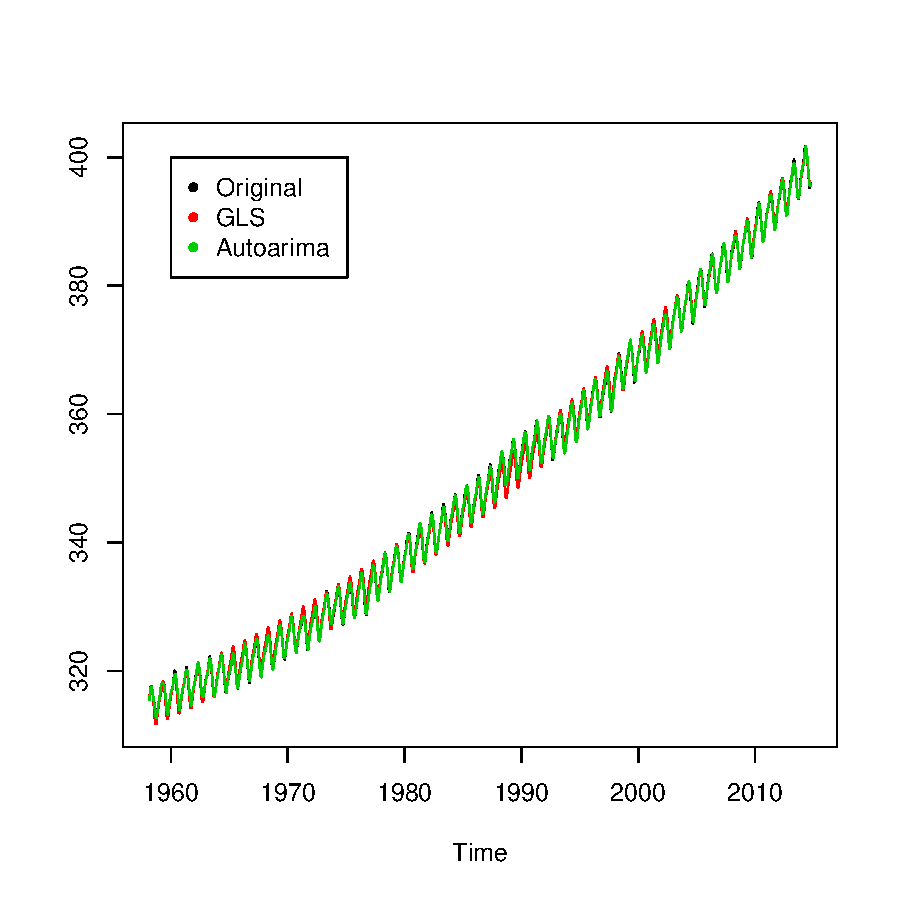
\includegraphics{FINAL_VERSION-fittedarima}
\caption{Fitted ARIMA values on time series}
\label{fittedarima}
\end{figure}


The comparison plot ~/ref{fittedarima} shows that the bestmodel from gls() and the automatically adjusted arima model are barely distinguishable from the original dataset. However, the arima gives slightly better AIC than the best gls. 

\begin{Schunk}
\begin{Sinput}
> AIC(autoarima)
\end{Sinput}
[1] 312.9221\end{Schunk}


\begin{figure}[ht]
\begin{center}
\subfloat[ACF]{
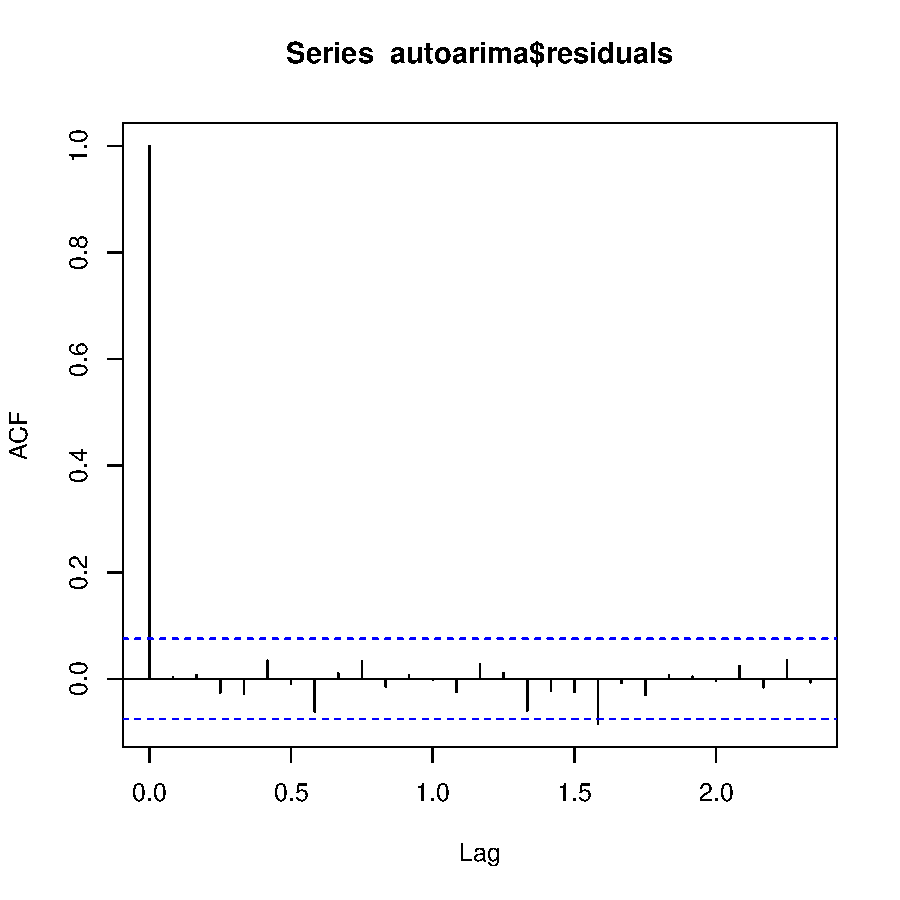
\includegraphics[width=0.3\textwidth]{FINAL_VERSION-arimaACF.pdf}
}
\qquad
\subfloat[PACF]{
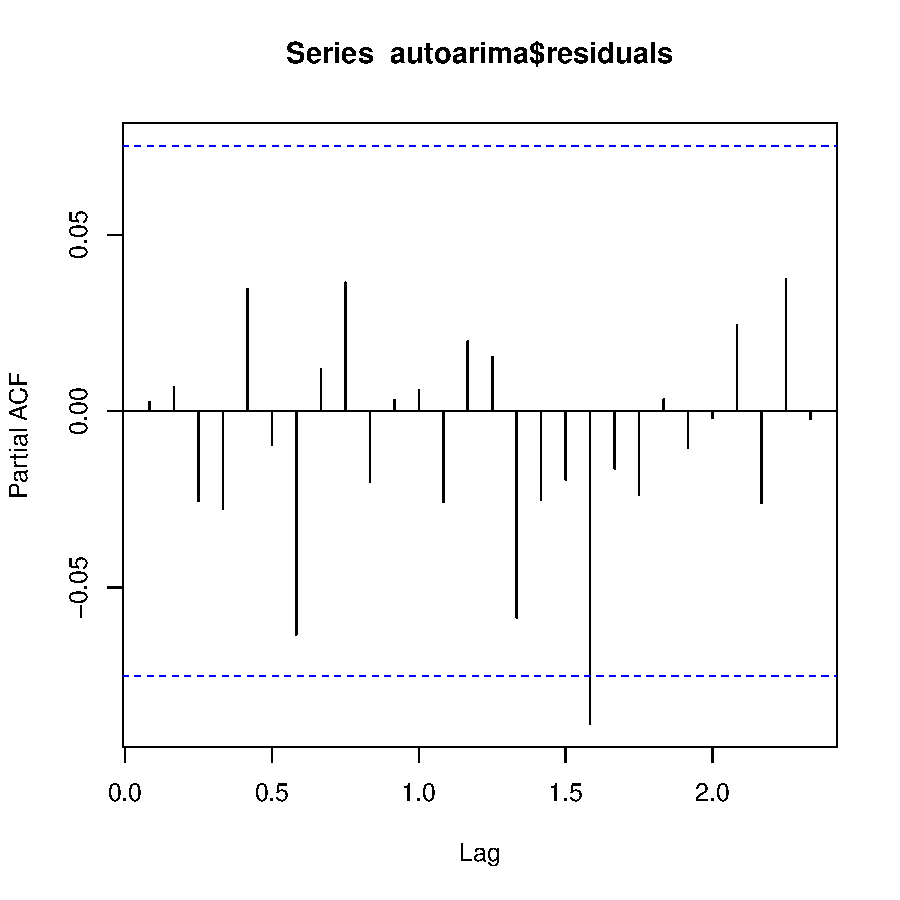
\includegraphics[width=0.3\textwidth]{FINAL_VERSION-arimaPACF.pdf}
}
\qquad
\subfloat[quadrARMA]{
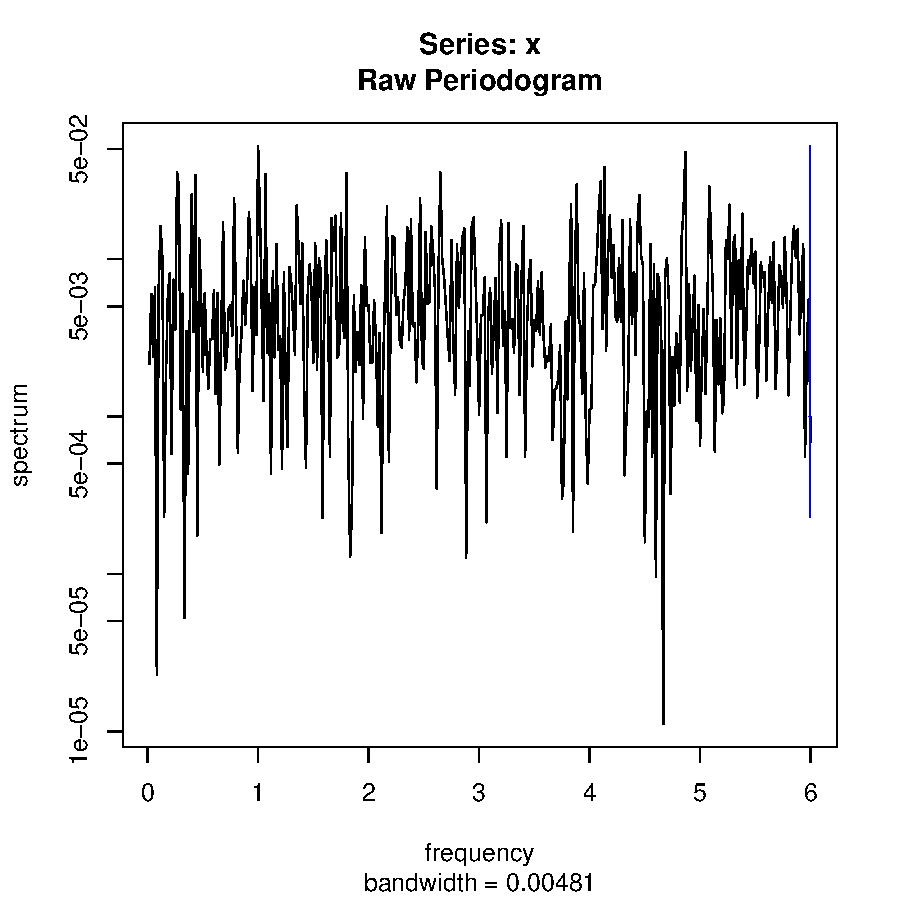
\includegraphics[width=0.3\textwidth]{FINAL_VERSION-arimaspec.pdf}
}
\end{center}
\caption{Correlogram for ARIMA}
\label{corarima}
\end{figure}



\begin{figure}[H]
\begin{center}
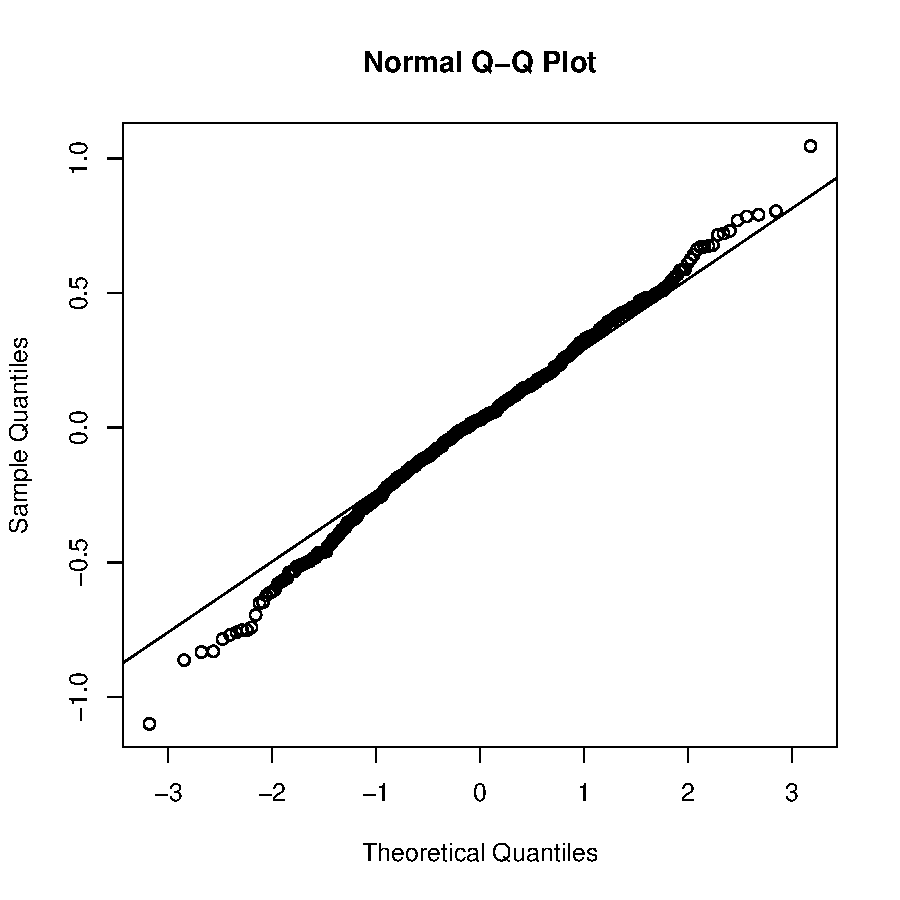
\includegraphics[width=0.5\textwidth]{FINAL_VERSION-qqarima.pdf}
\caption{QQ Plot for ARIMA}
\label{qqarima}
\end{center}
\end{figure}

\begin{Schunk}
\begin{Sinput}
> diagnostics(autoarima)
\end{Sinput}
\begin{Soutput}
     normality  stat.res stat.res.alt autocorr          
[1,] "0.037855" "0.01"   "stationary" "1.97955655809946"
     indep     
[1,] "0.946122"
\end{Soutput}
\end{Schunk}

The diagnostics show a better estimate of our fitted model. 
The autocorrelation is solved way better than in the gls-model. Also the stationarity is given now and the fitted values are independend. 



\section{Forecasts}%----------------------------------------------------------------------------------------------------
Forecasting means generally to predict from past values (x1,x2,x3,...,xn) some future values x(n+k). \\

We can choose from three different options: 
\begin{enumerate}
\item predict()
\item Holt Winters hw()
\item Arima forecasts forecast.Arima()
\end{enumerate}

If we have a time series that can be described using an additive model,we can short-time forecast using exponential smoothing.\\
A conditions we need to check are the forecast errors distributions. They need to be uncorrelated and normally distributed with mean zero and constant variance. To check the forecast errors we have the visualization of the function plotForecastErrors from above. 

\subsection{Forecast with predict()}
We use our best gls-model for this, the poly-2 model with SIN-COS-wave and predict for 10 years from the last period given in the data. 

\begin{Schunk}
\begin{Sinput}
> newtime= ts(start=c(2014, 10),end=c(2024,12),deltat=1/12)
> pred = predict(harmonizedARMAgls, newdata=newtime, se=T) 
> TIME <- as.numeric(time)
> time.df <- data.frame(TIME=TIME, COS, SIN)
> colnames(time.df)[-1] <- paste0("V", 1:12)
> smoothed <- gls(as.numeric(yourts) ~ TIME + I(TIME^2) + V1 + V2 + V3 + V4 + V5 
                 +V6 +V7+V8 +V9 +V10 +V11 +V12, 
                 corr=corAR1(acf(dataseasongls$residuals)$acf[2]),
                 data=time.df)
> new.df <- cbind.data.frame(TIME=as.numeric(time(newtime)), 
                            COS=COS[1:123,], SIN=SIN[1:123,])
> colnames(new.df)[-1] <- paste0("V", 1:12)
> pred = predictSE(smoothed, newdata=new.df, se.fit=T)
\end{Sinput}
\end{Schunk}

\begin{Schunk}
\begin{Sinput}
> plot(yourts, type="n",las=1, xlim=c(1960, 2025), 
      ylim=c(300, 450), xlab="Year", ylab="CO2 conc. (ppm)", 
      main="CO2 concentration in the atmosphere")
> grid (NULL,NULL, lty = 6, col = "cornsilk2") 
> points(yourts ,type="l" )
> par(mfrow=c(1,1))
> lines(as.numeric(time(newtime)), pred$fit, col="red")
> F=(pred$fit)
> FSUP=(pred$fit+1.96*pred$se.fit) # make upper conf. int. 
> FSLOW=(pred$fit-1.96*pred$se.fit) # make lower conf. int. 
> lines(new.df$TIME, FSUP,lty=1, col="grey", lwd=3)
> lines(new.df$TIME, FSLOW,lty=1, col="grey", lwd=3)
> lines(new.df$TIME, F, lty=1, col="red", lwd=1)
> legend("topleft",c("forecast for 10 years", "monthly mean data", "CI"), 
        pch=c(20,20), col=c("red", "black", "grey"))
\end{Sinput}
\end{Schunk}
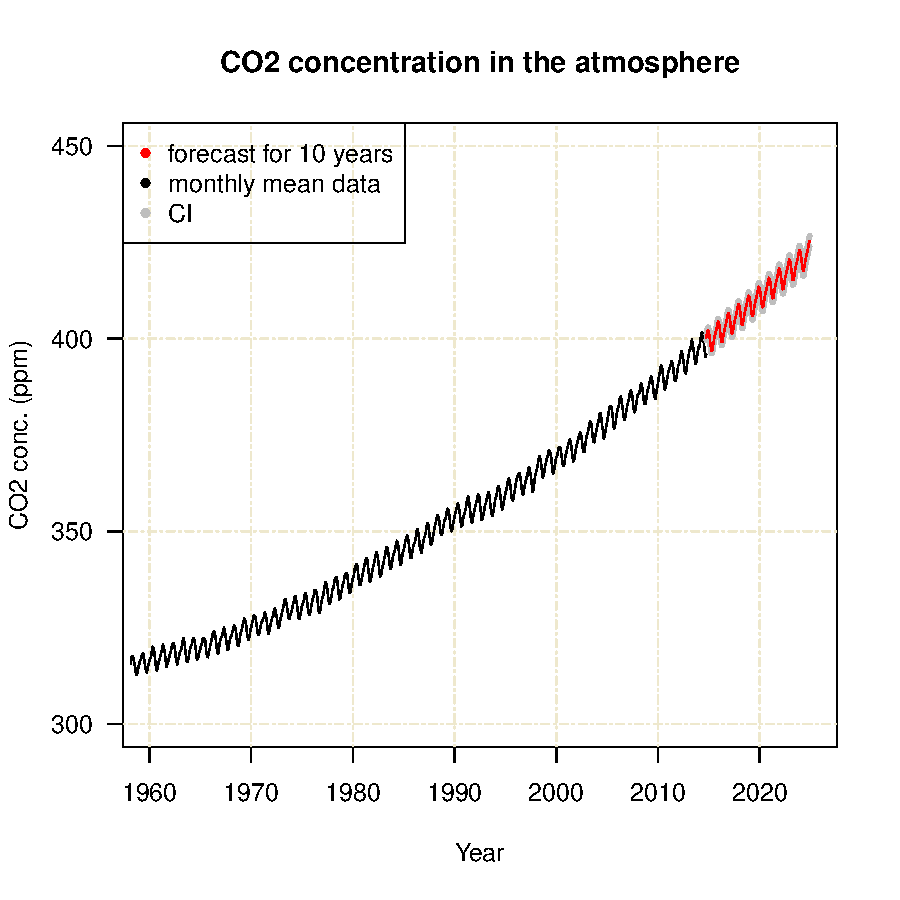
\includegraphics{FINAL_VERSION-067}


\subsection{Holtwinters forecast function}
The alpha value tells us the weight of the previous values for the forecasting. Gamma is used for the seasonality. Values of alpha that are close to 0 mean that little weight is placed on the most recent observations when making forecasts of future values and that the predicted values are highly smoothed estimates. If alpha is near 1, little smoothing is done and the estimates are at approximately previous xt. \\

It is important not to specify aphla, beta, gamma in order to include errors, trend and seasonal component in the forecast.We use the original data for hw() and predict in the period of 120*1 month = 10 years. Subsequently, we plot the predicted values with the original data and check the diagnostics.  \\
\begin{Schunk}
\begin{Sinput}
> forecast <- HoltWinters(yourts)
> forecast10 <- forecast.HoltWinters(forecast,h=120)
\end{Sinput}
\end{Schunk}

\begin{Schunk}
\begin{Sinput}
> par(mfrow=c(1,1))
> plot.forecast(forecast10,shadecols = "oldstyle")
\end{Sinput}
\end{Schunk}


\begin{Schunk}
\begin{Sinput}
> par(mfrow=c(2,1))
> acf(forecast10$residuals)
> pacf(forecast10$residuals)
\end{Sinput}
\end{Schunk}
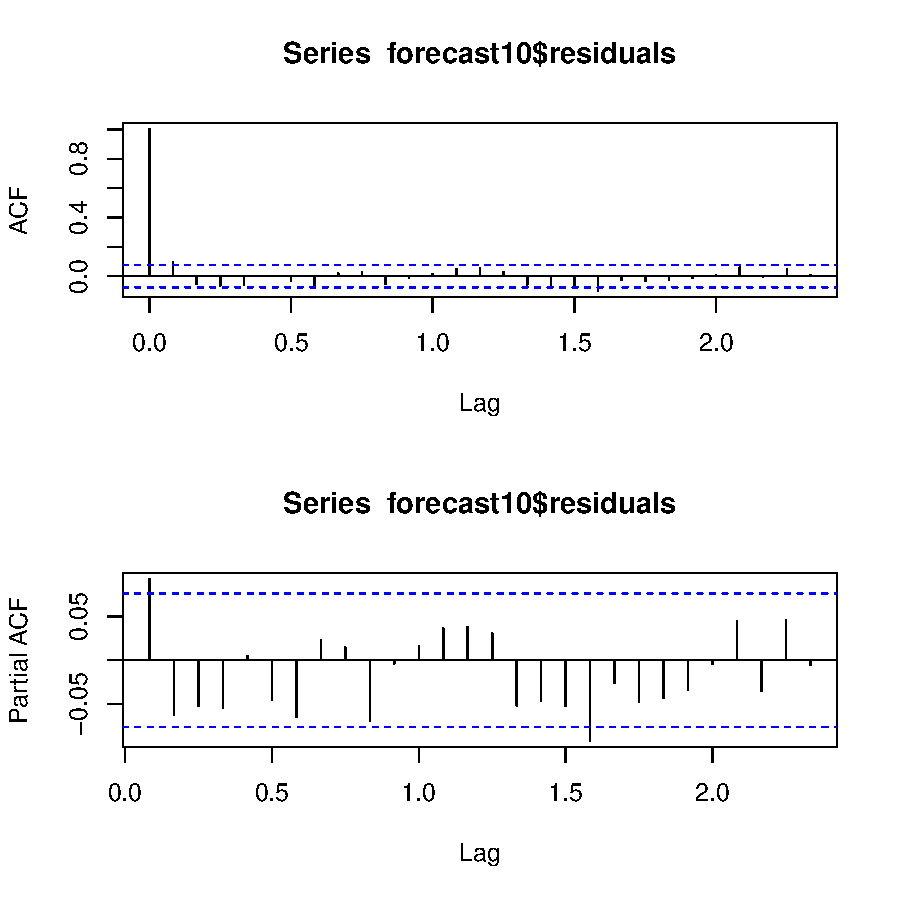
\includegraphics{FINAL_VERSION-070}

\subsection{ARIMA forecast function}
Now we try to forecast with the autoarima function as our bestmodel, which would save alot of time. 

\begin{Schunk}
\begin{Sinput}
> forecast.arima = forecast.Arima(autoarima, h=120) 
\end{Sinput}
\end{Schunk}

\subsection{Comparison of HW and ARIMA}
Now we can compare which forecast function complies better.

First thing on our list is, that we need to check for error distribution with the plotForecastErrors function from above:

\begin{figure}[ht]
\begin{center}
\subfloat[hw()]{
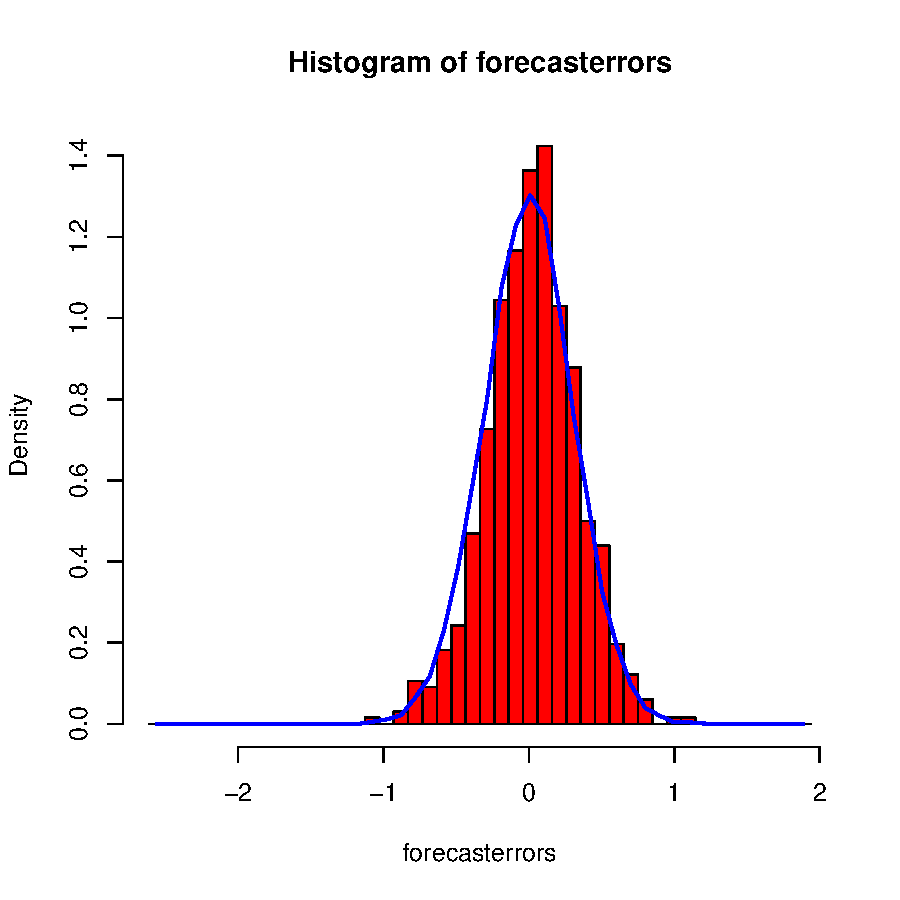
\includegraphics[width=0.3\textwidth]{FINAL_VERSION-forecasthwerr.pdf}
}
\qquad
\subfloat[arima]{
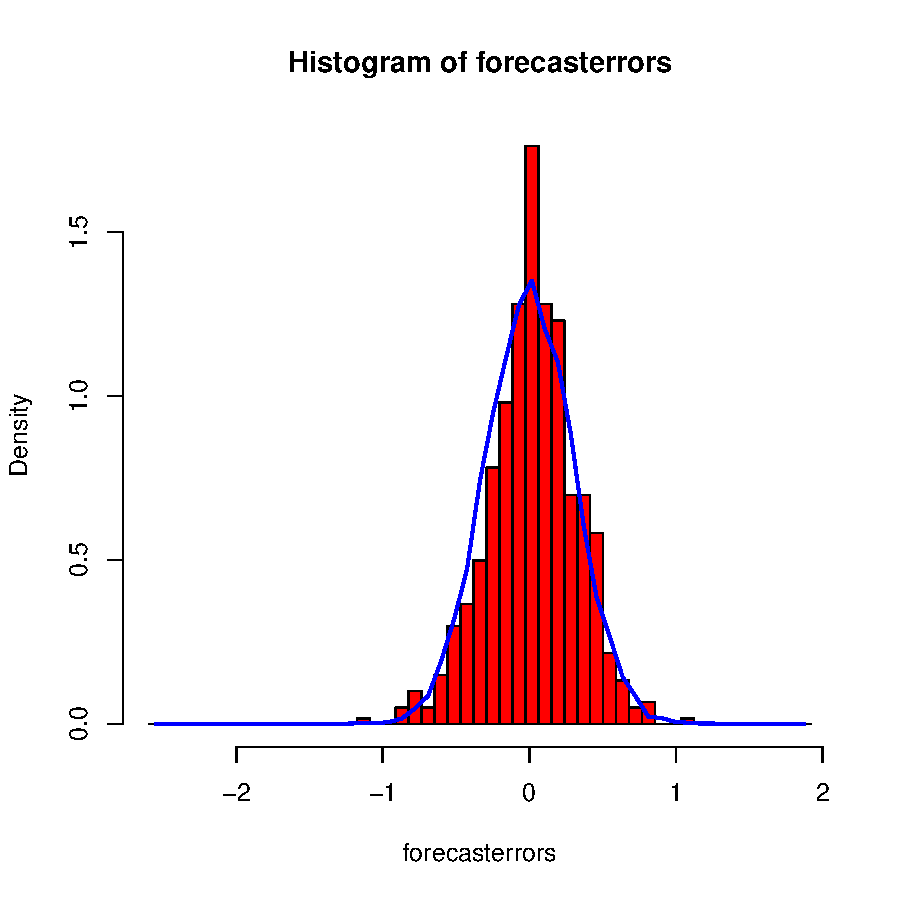
\includegraphics[width=0.3\textwidth]{FINAL_VERSION-arimaforerr.pdf}
}
\end{center}
\caption{Forcast error distribution}
\label{forerr}
\end{figure}

\noindent The histogram  of the time series in figure 21 shows that the forecast errors are roughly normally distributed and the mean seems to be close to zero for both functions.\\

Run diagnostics.\\
% latex table generated in R 3.1.1 by xtable 1.7-4 package
% Fri Nov 28 19:10:54 2014
\begin{table}[ht]
\centering
\begin{tabular}{rlllll}
  \hline
 & normality & stat.res & stat.res.alt & autocorr & indep \\ 
  \hline
1 & 0.357443 & 0.01 & stationary & 1.80314031521739 & 0.0174092 \\ 
   \hline
\end{tabular}
\caption{ Diagnostics hw-forecast} 
\end{table}% latex table generated in R 3.1.1 by xtable 1.7-4 package
% Fri Nov 28 19:10:54 2014
\begin{table}[ht]
\centering
\begin{tabular}{rlllll}
  \hline
 & normality & stat.res & stat.res.alt & autocorr & indep \\ 
  \hline
1 & 0.037855 & 0.01 & stationary & 1.97955655809946 & 0.946122 \\ 
   \hline
\end{tabular}
\caption{Diagnostics arima-forecast} 
\end{table}\linebreak

\noindent Through the diagnostics, we would choose the arima forecast as best forecast function. The values are independent, the autocorrelation is handled and we have stationarity. One problem is the not-normal distributed residuals, which the arima can take care of. In the hw() forecast we still have problems with the independence of the residuals. Both forecasts solved the more important problems of stationarity and autocorrelation. Now we can have a final look at both the forecast functions and also here, they are barely distinuigshable from each other. Both fit well.

\begin{figure}
\centering
\begin{Schunk}
\begin{Sinput}
> par(mfrow=c(2,1))
> plot(forecast.arima, xlim=c(2010,2025), ylim=c(385,430),shadecols = "oldstyle")
> plot.forecast(forecast10 ,xlim=c(2010,2025), ylim=c(385,430),shadecols = "oldstyle")
\end{Sinput}
\end{Schunk}
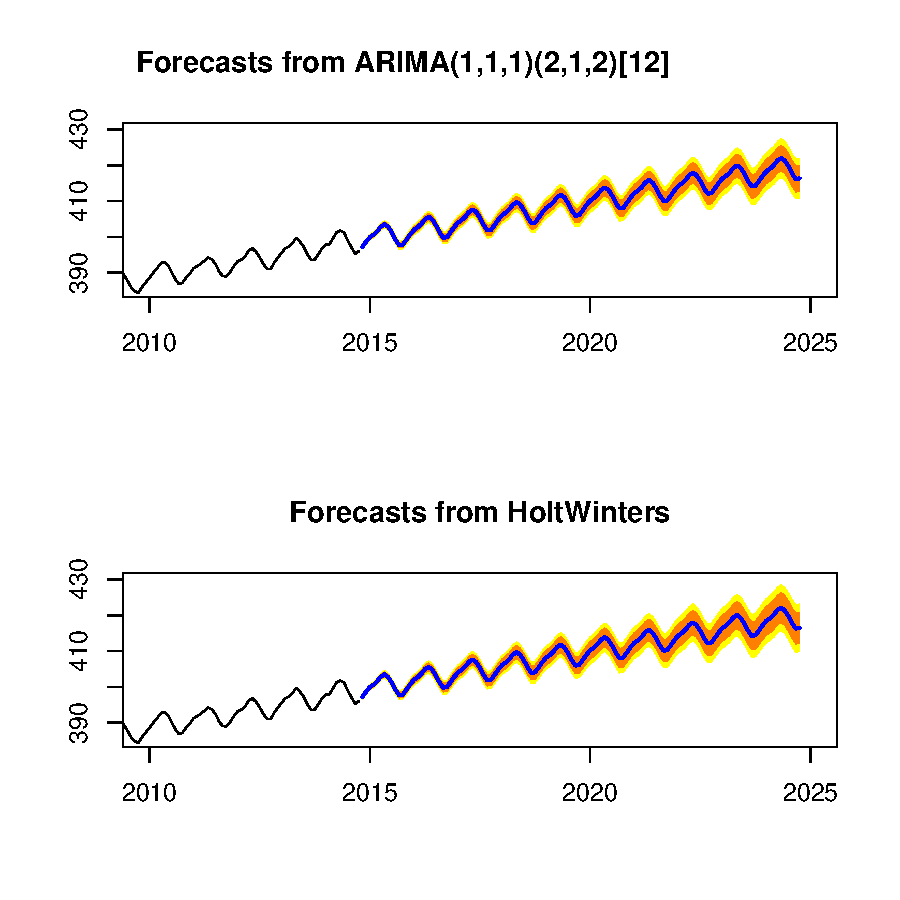
\includegraphics{FINAL_VERSION-075}
\caption{Comparison of different forecast functions}
\end{figure}

\subsection{Seasonal Decomposition of Time Series by Loess}

Forecasting using stl objects is a fourth option, which is straitforward using like hw() the original time series and plotting us nearly same results as other options.
\begin{figure}[H]
\centering
\begin{Schunk}
\begin{Sinput}
> plot(stlf(yourts, lambda=0, h =120))
> (tslm(yourts~time(yourts)))
\end{Sinput}
\begin{Soutput}
Call:
lm(formula = formula, data = "yourts", na.action = na.exclude)

Coefficients:
 (Intercept)  time(yourts)  
   -2618.494         1.494  
\end{Soutput}
\end{Schunk}
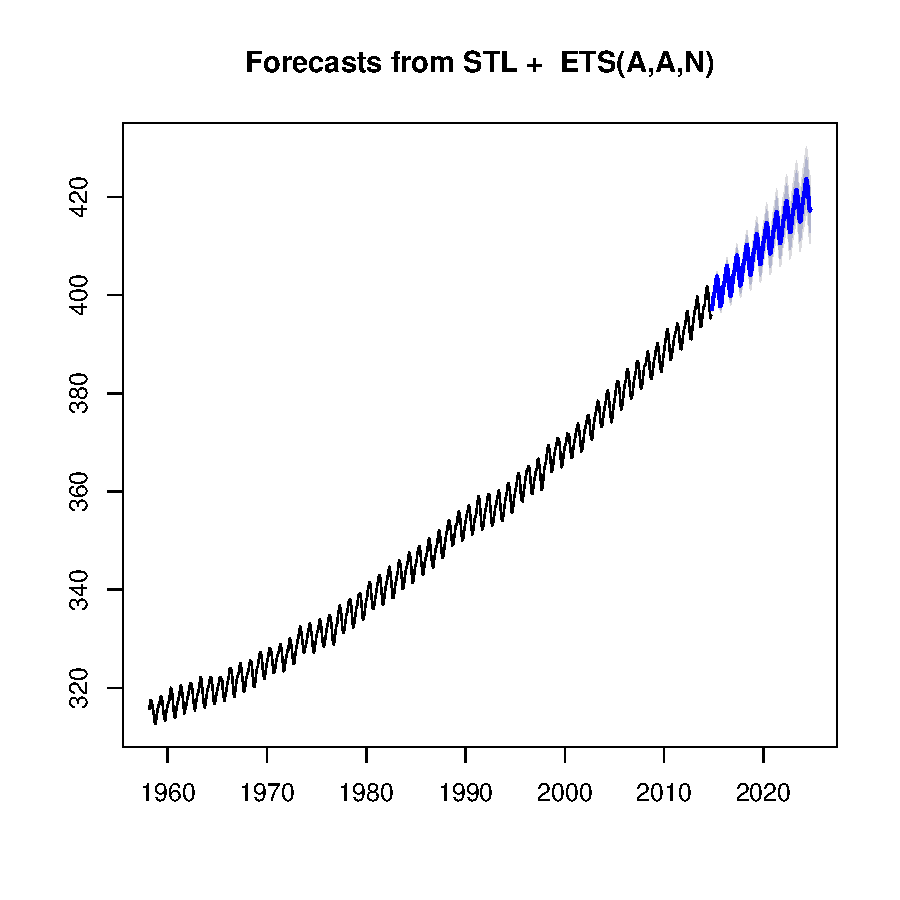
\includegraphics{FINAL_VERSION-076}
\caption{Forecasting using Loess}
\end{figure}


\subsection{Modelling time series with gam}

The gam() generalized additive model could maybe also help finding a quick solution for time series modelling. Thus this model is not adequately adjusted there are examples for modelling also seasonally components with gam(). We present it here and recommend further reading on it, for example on this website: http://www.fromthebottomoftheheap.net/2014/05/09/modelling-seasonal-data-with-gam/

\begin{Schunk}
\begin{Sinput}
> model = gam ( yourts ~ s(time))
\end{Sinput}
\end{Schunk}

\begin{Schunk}
\begin{Sinput}
> par(mfrow=c(1,1))
> plot.gam(model, residuals=T, scheme=c(2,1), all.terms=T)
\end{Sinput}
\end{Schunk}
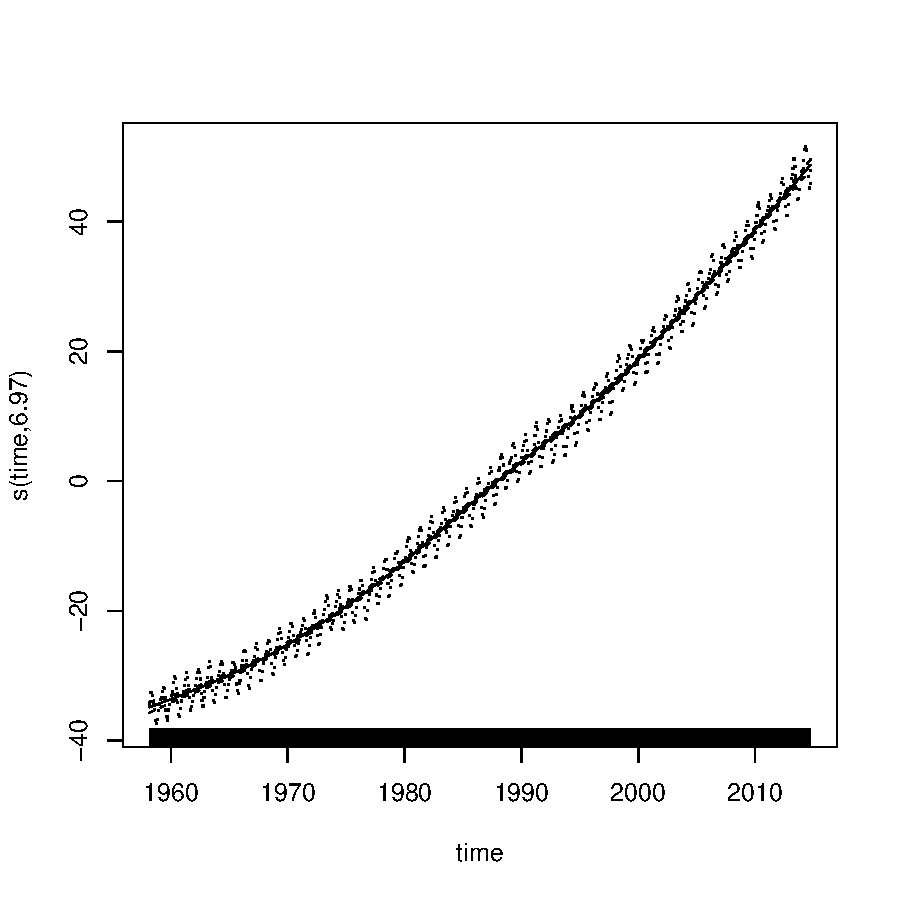
\includegraphics{FINAL_VERSION-078}

\begin{Schunk}
\begin{Sinput}
> smoothed4gam <- gam(as.numeric(yourts) ~ s(time)  +
                         COS[,1]+SIN[,1]+COS[,2]+SIN[,2]+
                         COS[,3]+SIN[,3]+COS[,4]+SIN[,4]+
                         COS[,5]+SIN[,5]+COS[,6]+SIN[,6]
                       , cor=corARMA(p=2, q=2))
> AIC(smoothed4gam)
\end{Sinput}
[1] 926.9626\end{Schunk}

\begin{figure}[H]
\centering
\begin{Schunk}
\begin{Sinput}
> plot(smoothed4gam)
> #8.91 is the edf:array of estimated degrees of 
> #freedom for the model terms, calculated for 
> #the smoothing term s(time)
\end{Sinput}
\end{Schunk}
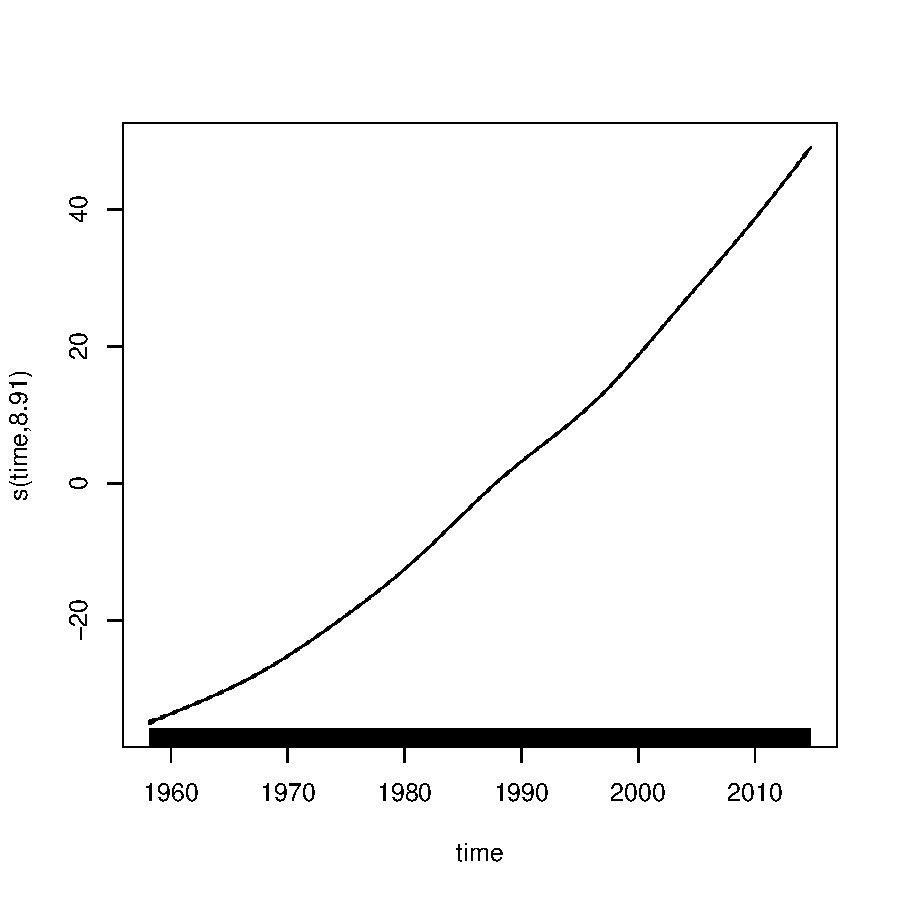
\includegraphics{FINAL_VERSION-080}
\caption{gam() with poly-1 smoothed term and sin-cos-wave}
\end{figure}


\section{Dataset Nile (Non-seasonal)}
\noindent Our example 2 contains the Measurements of the annual flow of the river Nile [m3/s] at Ashwan from 1871 to 1970. The Nile river data are included in any standard distribution of R as a time series object (i.e., a vector containing the data together with information about start/end time and sampling frequency); a detailed description of the data is given in the help file, ?Nile. \\
\\
First we visualize our data typing:

\begin{figure}[h!]
\centering
\begin{Schunk}
\begin{Sinput}
> plot(Nile, main="Annual flow of the Nile", ylab="Flow [m3/s]", xlab="years")
\end{Sinput}
\end{Schunk}
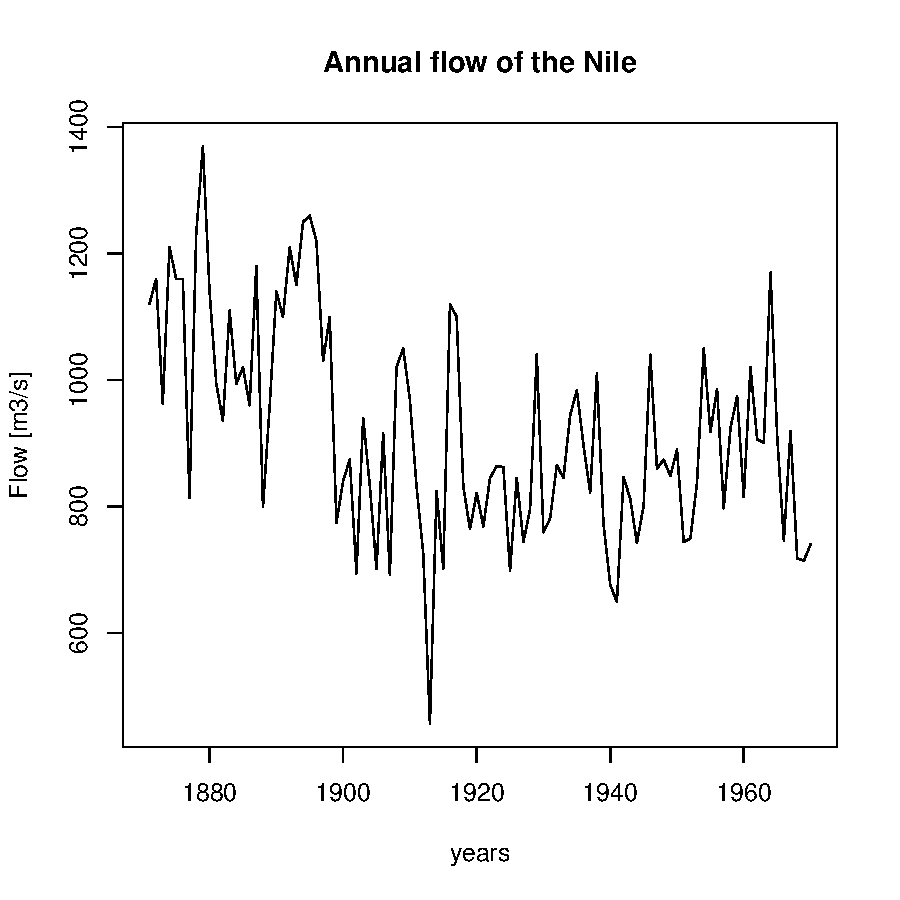
\includegraphics{FINAL_VERSION-081}
\caption{Annual Flow of the Nile}
\end{figure}
\begin{Schunk}
\begin{Sinput}
> class(Nile)
> str(Nile)
\end{Sinput}
\end{Schunk}

\noindent Since the time-series consists of annual observations, there are no indices of a cycle/seasonality in the data. A non-seasonal time series consists of a trend and an irregular component. 
To estimate the trend component of a non-seasonal time series that can be described using an additive model, it is common to use a smoothing method, such as calculating the simple moving average of the time series.

\noindent The SMA() function in the “TTR” R package can be used to smooth time series data using a simple moving average. 
\begin{figure}[H]
\centering
\begin{Schunk}
\begin{Sinput}
> library(TTR)
> sma = SMA(Nile)
> plot(SMA(Nile,n=20))
> 
\end{Sinput}
\end{Schunk}
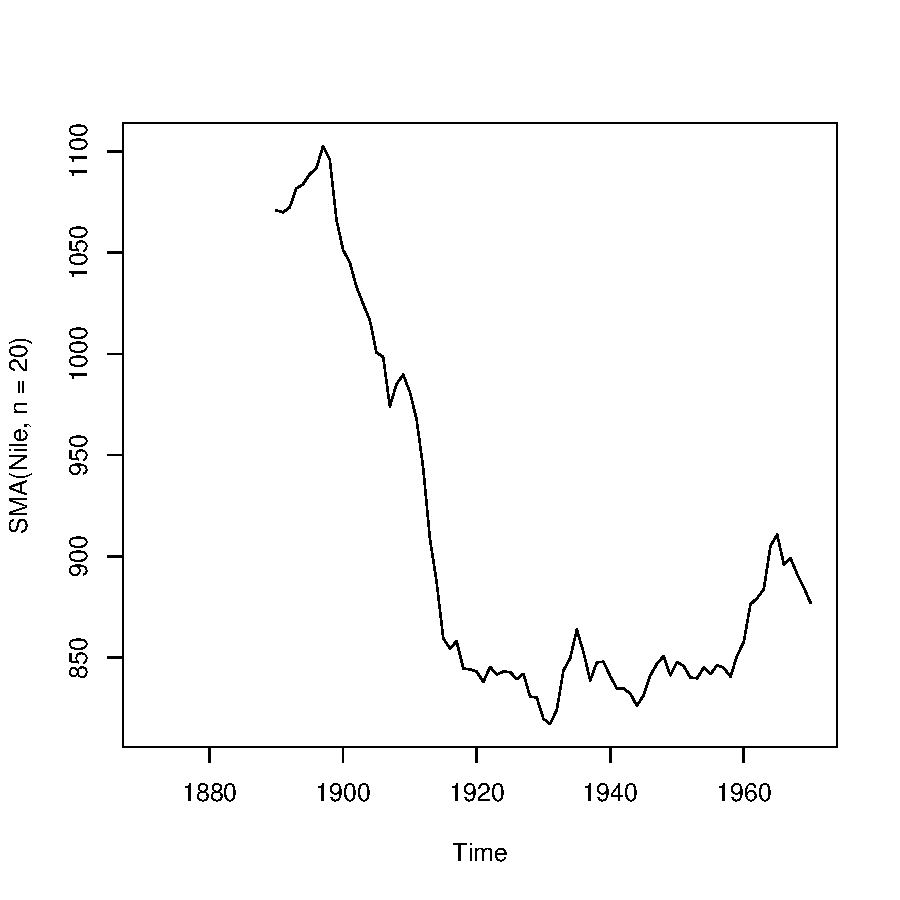
\includegraphics{FINAL_VERSION-083}
\caption{Trend of the Annual Flow of the Nile}
\end{figure}
\pagebreak
\noindent After using the SMA smoothing-function, we can clearly see that there was a negative trend until 1920 which was followed by a positive trend that reached its climax around 1965.until the end of the \\
\\
\noindent We can check if the data is stationary:
\begin{Schunk}
\begin{Sinput}
> adf.test(Nile)
\end{Sinput}
\begin{Soutput}
	Augmented Dickey-Fuller Test

data:  Nile
Dickey-Fuller = -3.3657, Lag order = 4, p-value =
0.0642
alternative hypothesis: stationary
\end{Soutput}
\begin{Sinput}
> kpss.test(Nile)
\end{Sinput}
\begin{Soutput}
	KPSS Test for Level Stationarity

data:  Nile
KPSS Level = 1.3152, Truncation lag parameter = 2,
p-value = 0.01
\end{Soutput}
\end{Schunk}
\\
\\
\\
The data is not stationary, we can conclude that the SMA-function was not appropriate for this time-series.\\
\\
\noindent We try to fit a linear model to the data:\\
\begin{Schunk}
\begin{Sinput}
> nilelm = lm(Nile~time(Nile))
> summary(nilelm)
\end{Sinput}
\begin{Soutput}
Call:
lm(formula = Nile ~ time(Nile))

Residuals:
    Min      1Q  Median      3Q     Max 
-483.71  -98.17  -23.21  111.40  368.72 

Coefficients:
             Estimate Std. Error t value Pr(>|t|)    
(Intercept) 6132.1736  1001.7578   6.121 1.92e-08 ***
time(Nile)    -2.7143     0.5216  -5.204 1.07e-06 ***
---
Signif. codes:  
0 '***' 0.001 '**' 0.01 '*' 0.05 '.' 0.1 ' ' 1

Residual standard error: 150.6 on 98 degrees of freedom
Multiple R-squared:  0.2165,	Adjusted R-squared:  0.2085 
F-statistic: 27.08 on 1 and 98 DF,  p-value: 1.072e-06
\end{Soutput}
\begin{Sinput}
> confint(nilelm)
\end{Sinput}
\begin{Soutput}
                  2.5 %      97.5 %
(Intercept) 4144.217893 8120.129266
time(Nile)    -3.749313   -1.679298
\end{Soutput}
\end{Schunk}

\begin{figure}[H]
\centering
\begin{Schunk}
\begin{Sinput}
> par(mfrow=c(1,2))
> acf(resid(nilelm))
> pacf(resid(nilelm))
\end{Sinput}
\end{Schunk}
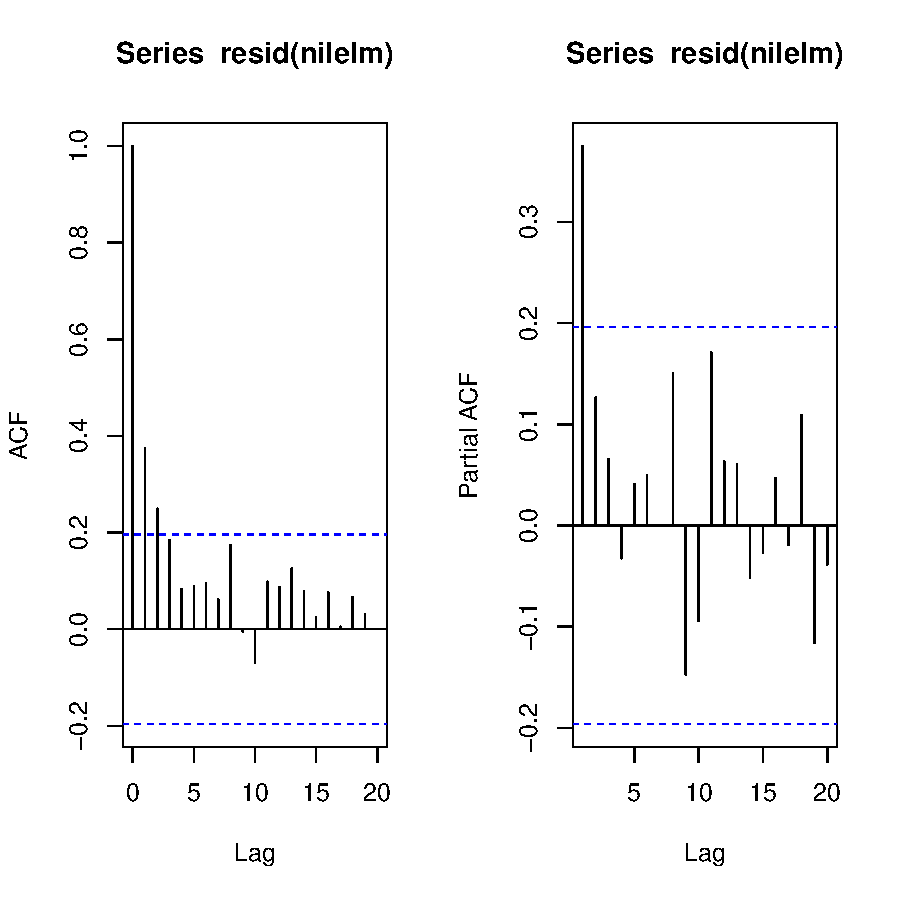
\includegraphics{FINAL_VERSION-086}
\caption{Autocorelations diagnostics of the Nile Time Series}
\end{figure}

\noindent We can see that the linear model is not appropriate,the correlograms indicate a positive autocorrelation in the first lags. Next we fit the gls function to provide better estimates to account for the autocorrelation in the residual series:\\
\begin{Schunk}
\begin{Sinput}
> nilegls = gls(Nile ~ time(Nile),cor= corAR1(acf(resid(nilelm))$acf[2]))
> save(nilegls, file="nilegls.RData")
\end{Sinput}
\end{Schunk}

\begin{Schunk}
\begin{Sinput}
> load("nilegls.RData")
\end{Sinput}
\end{Schunk}

\begin{Schunk}
\begin{Sinput}
> summary(nilegls)
\end{Sinput}
\begin{Soutput}
Generalized least squares fit by REML
  Model: Nile ~ time(Nile) 
  Data: NULL 
       AIC      BIC    logLik
  1268.205 1278.545 -630.1026

Correlation Structure: AR(1)
 Formula: ~1 
 Parameter estimate(s):
      Phi 
0.4002726 

Coefficients:
               Value Std.Error   t-value p-value
(Intercept) 6216.491 1518.1486  4.094784   1e-04
time(Nile)    -2.758    0.7904 -3.489523   7e-04

 Correlation: 
           (Intr)
time(Nile) -1    

Standardized residuals:
       Min         Q1        Med         Q3        Max 
-3.1787691 -0.6428562 -0.1463738  0.7245317  2.4323739 

Residual standard error: 152.3157 
Degrees of freedom: 100 total; 98 residual
\end{Soutput}
\begin{Sinput}
> confint(nilegls)
\end{Sinput}
\begin{Soutput}
                  2.5 %      97.5 %
(Intercept) 3240.974234 9192.007340
time(Nile)    -4.307301   -1.208971
\end{Soutput}
\end{Schunk}

\begin{figure}[h]
\centering
\begin{Schunk}
\begin{Sinput}
> acf(nilegls$residuals); pacf(nilegls$residuals)
\end{Sinput}
\end{Schunk}

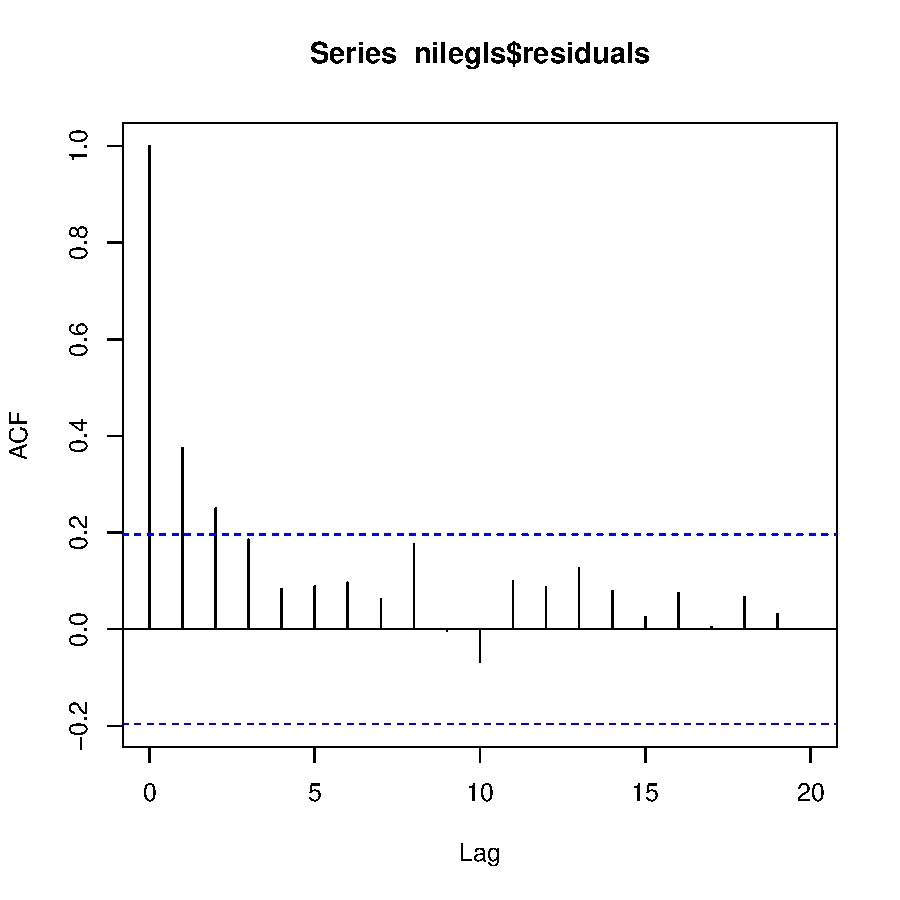
\includegraphics{FINAL_VERSION-090}
\caption{Autocorrelation diagnostics for the gls Model}
\end{figure}

\begin{figure}[h]
\centering
\begin{Schunk}
\begin{Sinput}
> plot(nilegls)
\end{Sinput}
\end{Schunk}
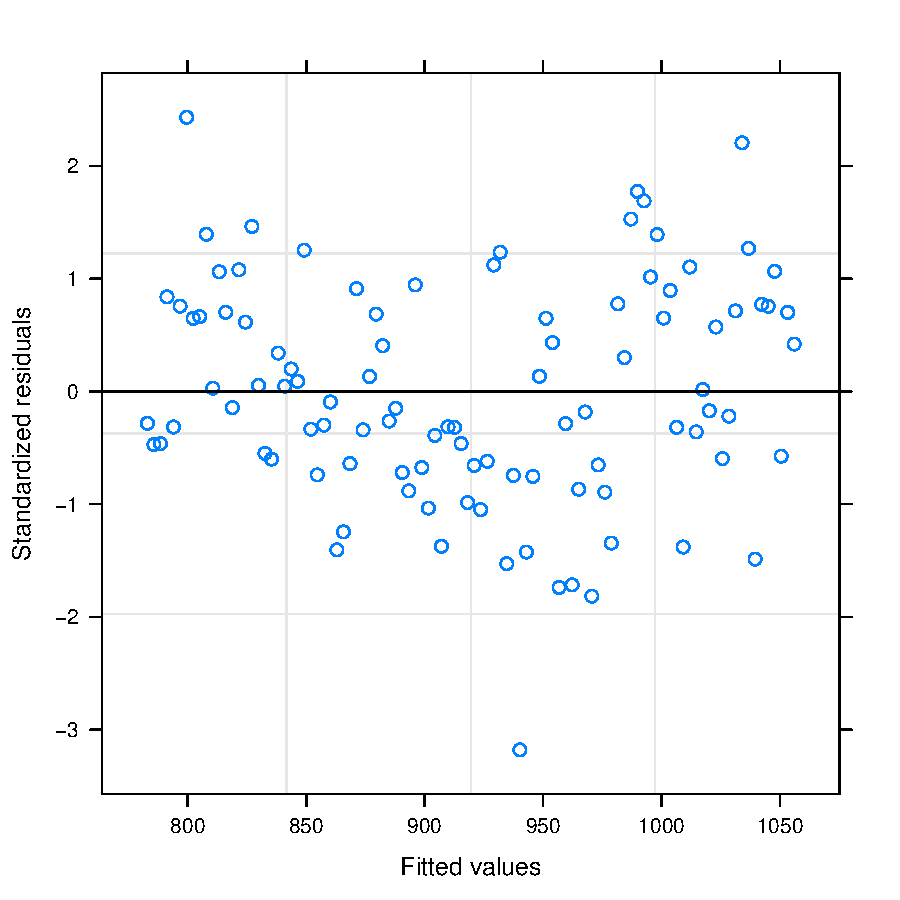
\includegraphics{FINAL_VERSION-091}
\caption{Residuals of the gls Model}
\end{figure}

\noindent The residuals look like white noise, next we test if they are independent:\\
\\
\begin{Schunk}
\begin{Sinput}
> Box.test(nilegls$residuals, type="Ljung-Box")
\end{Sinput}
\begin{Soutput}
	Box-Ljung test

data:  nilegls$residuals
X-squared = 14.496, df = 1, p-value = 0.0001405
\end{Soutput}
\end{Schunk}
\\
\noindent The null hypothesis is rejected, the residuals are not independent
(p<0.05).

% \begin{figure}[H]
% \centering
% <<fig=TRUE>>=
% arnile = ar(Nile) 
% acf(resid(arnile))
% cpgram(ar(Nile)$resid)
% 
% arima(Nile, c(2, 0, 0))
% 
% @
% \caption{Cumulative Peridiogram of the residuals}
% \end{figure}
% 
% \noindent Fitting a autoregressive model, we can see that the residuals are well placed.



\noindent We find a significant autocorrelation at the first lags only, that means that the autocorrelation decreases with the time. We see no indices of seasonality. 
The ACF does not show any significant autocorrelation. \textbf{INSERT ACF PICTURE}


\subsection{Holt Winters exponential smoothing}

\begin{figure}[H]
\centering
\begin{Schunk}
\begin{Sinput}
> library(forecast)
> hwn = HoltWinters(Nile,alpha = 0.2, beta = FALSE, gamma = FALSE,
                   start.periods =c(1120,740) )
> plot(hwn)
> 
\end{Sinput}
\end{Schunk}
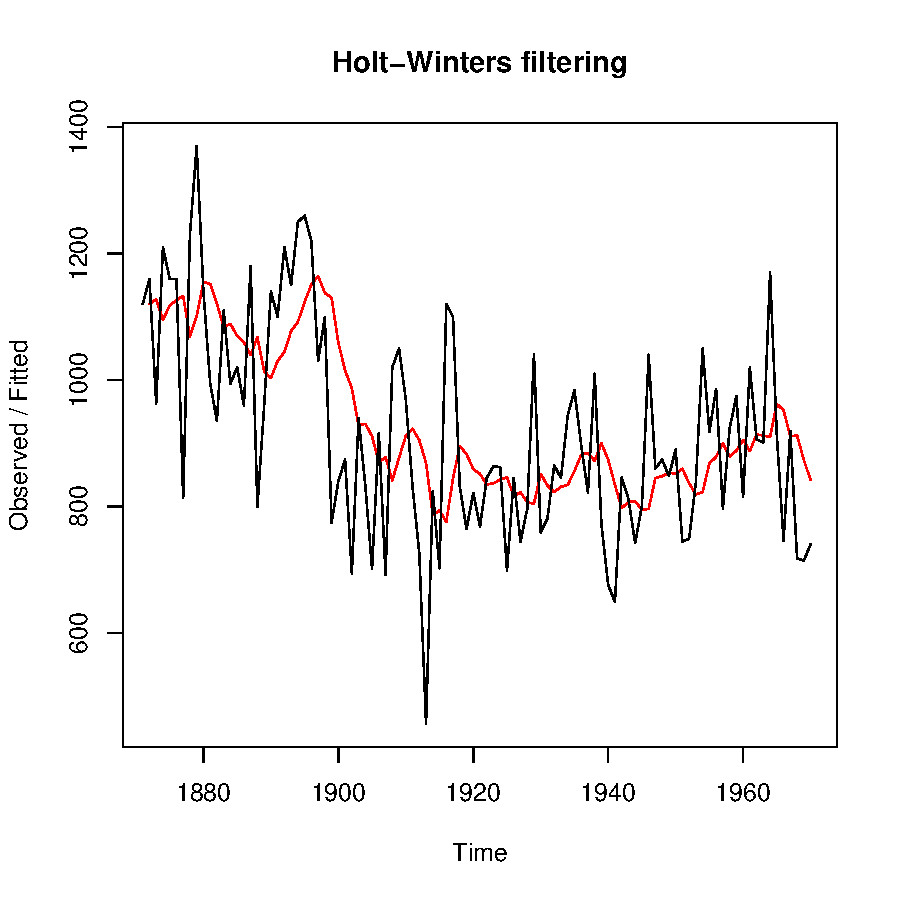
\includegraphics{FINAL_VERSION-093}
\caption{Holt Winters}
\end{figure}

\begin{figure}[H]
\centering
\begin{Schunk}
\begin{Sinput}
> forecast_nile = forecast.HoltWinters(hwn, h=5)
> plot.forecast(forecast_nile, shadecols = "oldstyle")
> 
\end{Sinput}
\end{Schunk}
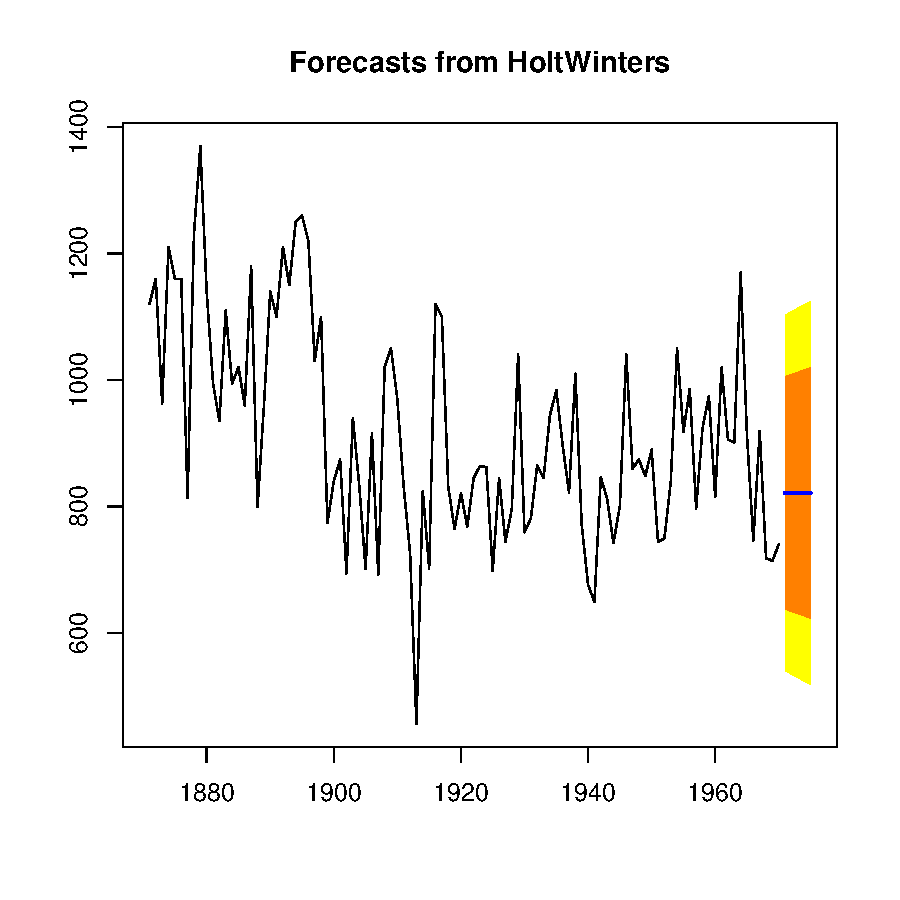
\includegraphics{FINAL_VERSION-094}
\caption{Holt Winter Forecasting}
\end{figure}

\noindent The forecasts are shown as a blue line, with the 80% prediction intervals as an orange shaded area, and the 95% prediction intervals as a yellow shaded area.


\begin{Schunk}
\begin{Sinput}
> acf(forecast_nile$residuals, lag.max = 20)
> pacf(forecast_nile$residuals, lag.max = 20)
> Box.test(forecast_nile$residuals, lag=20, type="Ljung-Box")
\end{Sinput}
\begin{Soutput}
	Box-Ljung test

data:  forecast_nile$residuals
X-squared = 15.8772, df = 20, p-value = 0.7242
\end{Soutput}
\begin{Sinput}
> 
\end{Sinput}
\end{Schunk}
\noindent The p-value of the Ljung-Box test (0.72) indicates that there is little evidence of non-zero autocorrelations in the in-sample forecast errors at lags 1-20. The residuals are now independent.\\

\noindent We should check if the forecast errors have constant variance over time, and are normally distributed with mean zero. We can do this by plotting the forecast errors and a histogram of the distribution of these errors.

\begin{figure}[H]
\centering
\begin{Schunk}
\begin{Sinput}
> par(mfrow=c(1,2))
> plot.ts(forecast_nile$residuals);abline(h=0)
> plotForecastErrors(forecast_nile$residuals)
> par(mfrow=c(1,1))
\end{Sinput}
\end{Schunk}
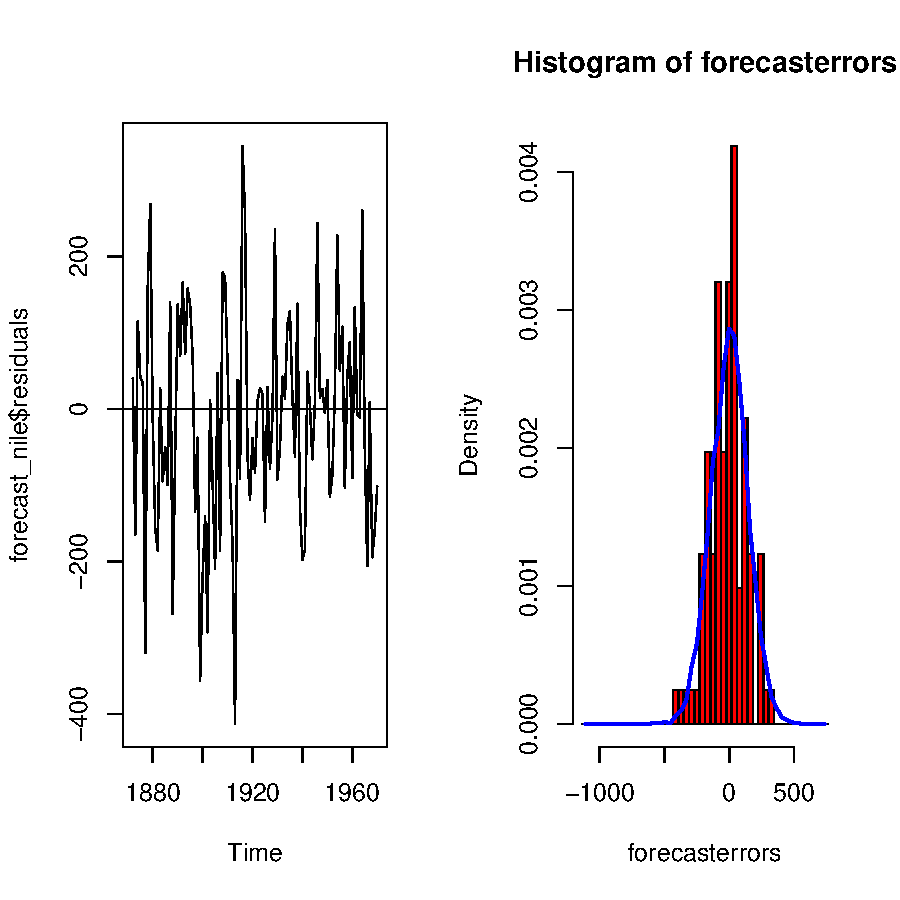
\includegraphics{FINAL_VERSION-096}
\caption{Forecast Errors}
\end{figure}

\noindent The forecast error plot shows roughly constant variance over time. The histogram of forecast errors emphasizes normally distributed residuals with mean zero and constant variance.

\subsection{ARIMA}

\noindent While exponential smoothing methods do not make any assumptions about correlations between successive values of the time series, in some cases you can make a better predictive model by taking correlations in the data into account. Autoregressive Integrated Moving Average (ARIMA) models include an explicit statistical model for the irregular component of a time series, that allows for non-zero autocorrelations in the irregular component.
\begin{figure}[H]
\centering
\begin{Schunk}
\begin{Sinput}
> nile_arima = auto.arima(Nile)
> forecast_nile2 = forecast.Arima(nile_arima, h=10)
> plot.forecast(forecast_nile2, shadecols = "oldstyle")
> 
\end{Sinput}
\end{Schunk}
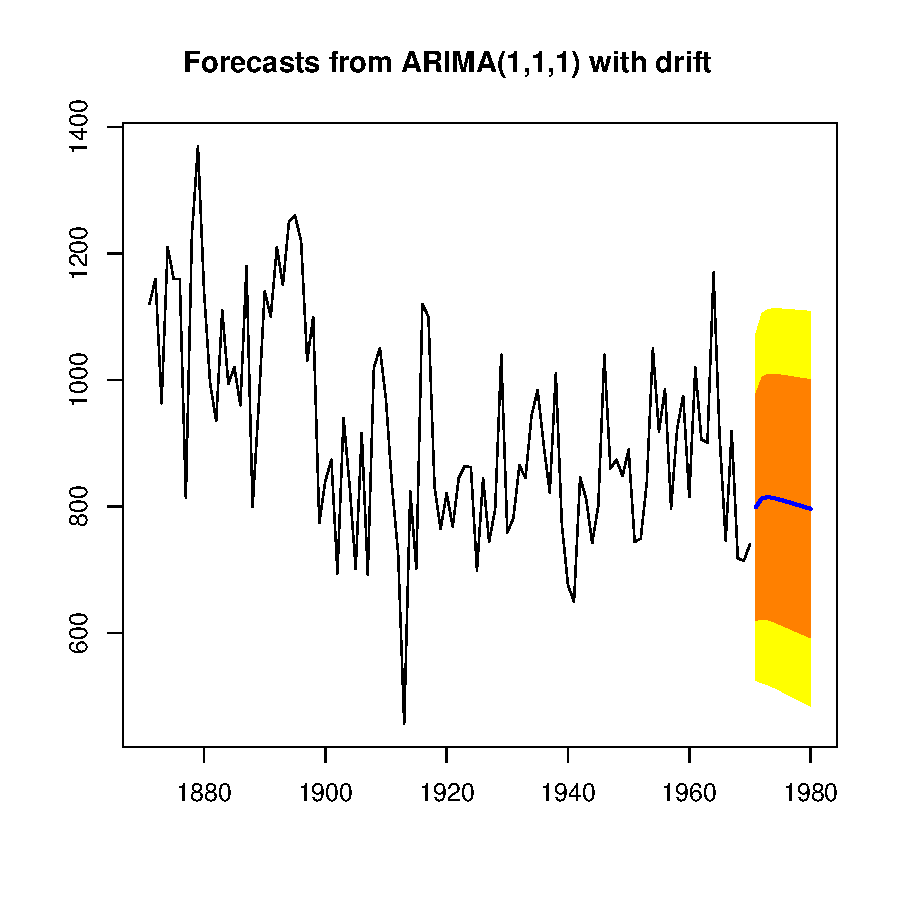
\includegraphics{FINAL_VERSION-097}
\caption{Arima forecasting}
\end{figure}

Check for autocorrelations:
\begin{figure}[H]
\centering
\begin{Schunk}
\begin{Sinput}
> acf(forecast_nile2$residuals, lag.max = 20)
> Box.test(forecast_nile2$residuals, lag=20, type="Ljung-Box")
\end{Sinput}
\begin{Soutput}
	Box-Ljung test

data:  forecast_nile2$residuals
X-squared = 12.1156, df = 20, p-value = 0.912
\end{Soutput}
\end{Schunk}
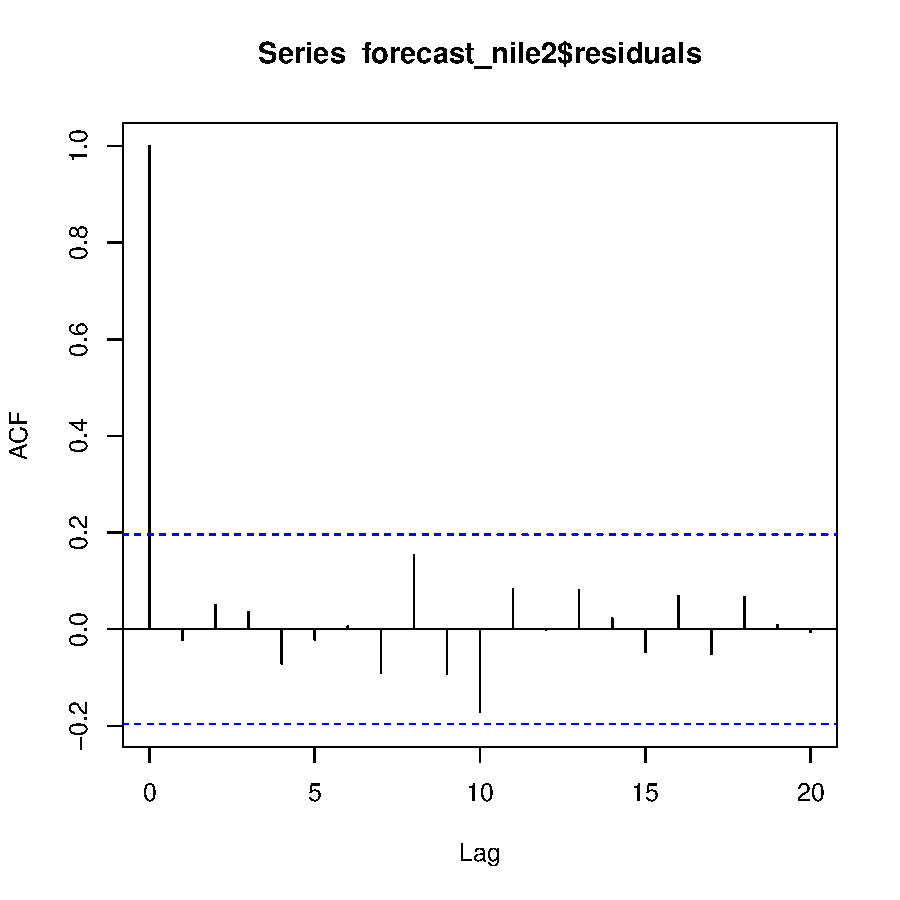
\includegraphics{FINAL_VERSION-098}
\caption{acf of the residuals}
\end{figure}
\noindent There is little evidence of non-zero autocorrelations in the in-sample forecast errors at lags 1-20. The residuals are now independent and the autocorrelation plots look nice.

\begin{figure}[H]
\centering
\begin{Schunk}
\begin{Sinput}
> par(mfrow=c(1,2))
> plot.ts(forecast_nile2$residuals); abline(h=0)
> plotForecastErrors(forecast_nile2$residuals)
\end{Sinput}
\end{Schunk}
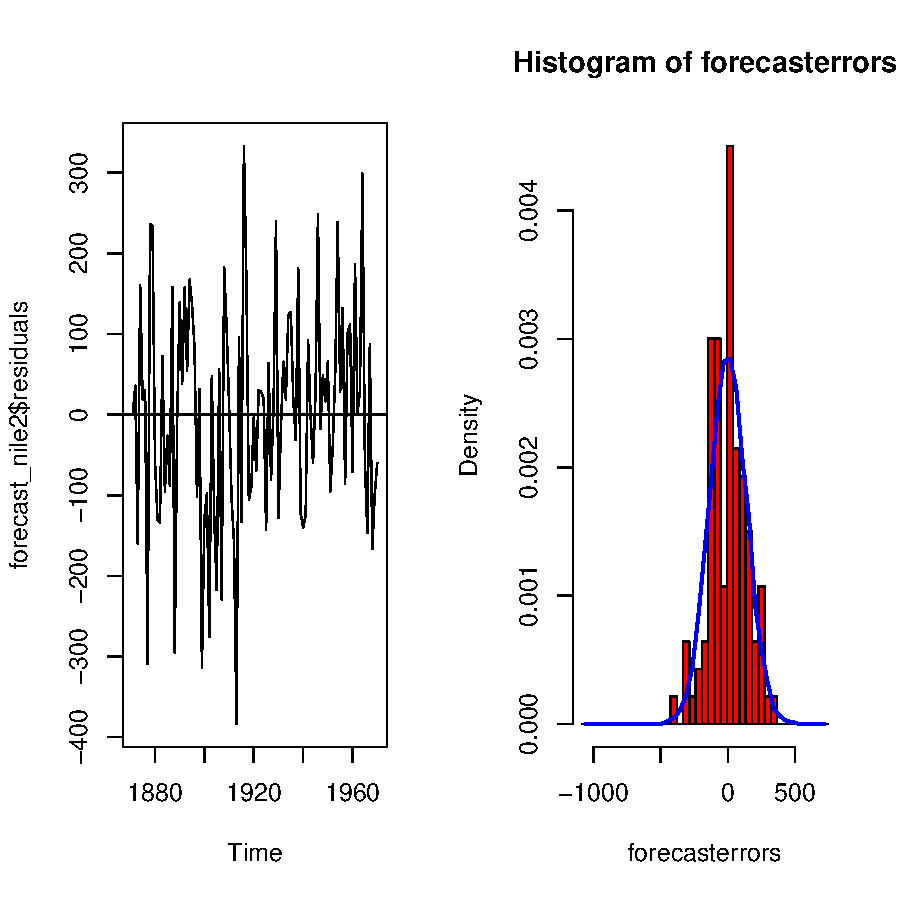
\includegraphics{FINAL_VERSION-099}
\caption{Residuals and Errors}
\end{figure}


\noindent We run a Durbin Watson Test to check for autocorrelations:
\begin{Schunk}
\begin{Sinput}
> library(car)
> dwt(as.vector(nilegls$residuals)) 
\end{Sinput}
\begin{Soutput}
[1] 1.247133
\end{Soutput}
\end{Schunk}
\noindent The Durbin Watson Test of the residuals shows that there is no autocorrelation and the residuals are independent.


\subsection{Structural time series models}

\noindent The function StructTS fits a model by maximum likelihood.
\begin{Schunk}
\begin{Sinput}
> fit <- StructTS(Nile, type = "level")
> fit
\end{Sinput}
\begin{Soutput}
Call:
StructTS(x = Nile, type = "level")

Variances:
  level  epsilon  
   1469    15099  
\end{Soutput}
\end{Schunk}
\noindent The Maximum Likelihood Estimates (MLEs) of the level- and observation error variances, 1469 and 15099, respectively, are included in the output as the coefficients of fit. 
\begin{figure}[H]
\centering
\begin{Schunk}
\begin{Sinput}
> par(mfrow = c(3, 1))
> plot(Nile)
> # local level model (contemporaneous smoothing)
> lines(fitted(fit), lty = "dashed", col=4) 
> # fixed-interval smoothing
> lines(tsSmooth(fit), lty = "dotted", col = 6) 
> legend("bottomright" ,col = c(4,6),c("filtered","smoothed"),
        lty=c("dashed", "dotted"), bty="n", cex=0.8)
> plot(residuals(fit)); abline(h = 0, lty = 3)
> # local trend model (constant trend fitted)
> fit2 <- StructTS(Nile, type = "trend")
> pred <- predict(fit, n.ahead = 30)
> # with 95% confidence interval
> ts.plot(Nile, pred$pred,
         pred$pred + 1.96*pred$se, pred$pred -1.96*pred$se,
         col=c(1,2,1))
> par(mfrow=c(1,1))
> 
\end{Sinput}
\end{Schunk}
\includegraphics{FINAL_VERSION-102}
\caption{Fitting a Structural Model}
\end{figure}

\noindent The function (tsdiag) can be called on an object of class StructTS to obtain diagnostic plots based on the standardized one-step-ahead forecast errors.
\begin{figure}[H]
\centering
\begin{Schunk}
\begin{Sinput}
> tsdiag(fit)
> tsdiag(fit2)
> 
\end{Sinput}
\end{Schunk}
\includegraphics{FINAL_VERSION-103}
\caption{Models diagnostics}
\end{figure}

\begin{figure}[H]
\centering
\begin{Schunk}
\begin{Sinput}
> library(forecast)
> plot(forecast(fit2, level = c(50,90), h = 10), xlim = c(1950, 1980), 
      shadecols = "oldstyle")
\end{Sinput}
\end{Schunk}
\includegraphics{FINAL_VERSION-forecasted_values}
\caption{Forecasted values}
\label{forecast_values}
\end{figure}

\noindent Forecasts for structural time series, as objects of class StructTS, can be obtained by either the method function (predict) or (forecast) in package forecast (Hyndman 2011; Hyndman and Khandakar 2008). This package also provides a convenient plot method function for the resulting object of class forecast. The plot of forcasted values, obtained with the code below, shows the forecasted Nile river data until 1980, togeher with 50\% and 90\% probability intervals.

\subsection{The package dlm and the Kalman filter}
\noindent A polynomial DLM (a local level model is a polynomial DLM of order 1, a local linear trend is a polynomial DLM of order 2), is easily defined in dlm through the function (dlmModPoly).The function simulates one draw from the posterior distribution of the state vectors.

\begin{figure}[H]
\centering
\begin{Schunk}
\begin{Sinput}
> library(dlm)
> nile_mod <- dlmModPoly(1, dV = 15099.8, dW = 1468.4)
> #values taken from the coefficients of fit
> nile_filt <- dlmFilter(Nile, nile_mod)
> nile_smooth <- dlmSmooth(nile_filt) # estimated "true" level
> plot(cbind(Nile, nile_smooth$s[-1]), plot.type = "s",
      col = c("black", "red"), ylab = "Level",
      main = "Nile river", lwd = c(2, 2)) 
> for (i in 1:10) # 10 simulated "true" levels 
     lines(dlmBSample(nile_filt[-1]), lty=2, col= "mediumblue"   )
\end{Sinput}
\end{Schunk}
\includegraphics{FINAL_VERSION-105}
\caption{dlm Model}
\end{figure}

\subsection{GAM (Generalized Additive Model)}
\begin{figure}[H]
\centering
\begin{Schunk}
\begin{Sinput}
> library(mgcv)
> niletime = time(Nile)
> gamnile = gam(as.numeric(Nile) ~ s(niletime),cor=corARMA(p=2, q=0))
> plot.gam(gamnile,residuals = T, se=T, main="GAM-Model", shade = T,
          seWithMean = T, all.terms = T , cex=2 )
\end{Sinput}
\end{Schunk}
\includegraphics{FINAL_VERSION-106}
\caption{GAM Model}
\end{figure}

\noindent We can now check which model has the best AIC:
\begin{Schunk}
\begin{Sinput}
> AIC(nilelm)
\end{Sinput}
\begin{Soutput}
[1] 1290.629
\end{Soutput}
\begin{Sinput}
> AIC(nilegls)
\end{Sinput}
\begin{Soutput}
[1] 1268.205
\end{Soutput}
\begin{Sinput}
> AIC(nile_arima)
\end{Sinput}
\begin{Soutput}
[1] 1254.913
\end{Soutput}
\begin{Sinput}
> AIC(gamnile)
\end{Sinput}
\begin{Soutput}
[1] 1274.499
\end{Soutput}
\end{Schunk}
\noindent The nile\_arima Model seems to be the best one.


\section{Compabitily with Linux and Windows}
\noindent We as a group experienced a lot of compatibility problems between Linux and Windows users when working on the same sweave document. If you also deal with line break issues or other unexplainable errors, one possible option to fix this is by transforming your Linux sweave document with the terminal command \enquote{unix2dos yourfilename.Rnw}.



\pagebreak
\section{Conclusion and helpful links}

Reminding of the Socratic paradox \enquote{I know one thing: that I know nothing} , we recommend further reading on the topic of time series. As we were noticing while dealing with the different correlation structures, our tutorial is considering the time series which are temporally autocorrelated. There are other covariance structures needed if you have spatially autocorrelated time series. \\

Helpful links for further reading: \\

\textbf{Time-Series Analysis in R:}
\\
http://cran.r-project.org/web/views/TimeSeries.html\\
\\
\textbf{Additional Example-Datasets:}
\\
http://www.comp-engine.org/timeseries/browse-data-by-category\\
https://datamarket.com/data/list/?q=provider:tsdl\\
\\
\textbf{Introductory Time Series with R:} Book by Cowpertwait and Metcalfe (Springer 2009)\\
\\

\section{Acknowledgements}%------------------------------------------------------------------------------------------------------
We like to thank the whole TeX and R community for providing us with an incredible amount of open source software. Without You this tutorial would have never been created!

\end{document}

